% !TEX program = xelatex
%% =====================================================================================================
%% NeuroChip Twin v2 -- technical report (TEMPLATE).
%%
%% Numbers: every numeric result is a double-brace token (file.json : dotted.path | format) resolved from
%% repo/results/*.json by scripts/render_docs.py, which writes report/neurochip_twin_v2.tex and the
%% number ledger (docs/NUMBERS.md, results/numbers_ledger.json). Never type a result by hand. Literal
%% numbers in this file are structural constants only (17 features, DIV 5/7/9/12, 48-well plates, grid
%% values and thresholds fixed a priori in the protocols, rubric weights, dates, identifiers).
%%
%% Build:  python scripts/render_docs.py
%%         cd report && xelatex neurochip_twin_v2 && biber neurochip_twin_v2 && xelatex ×2
%% Figures: report/figures/<stem>.pdf (vector) + <stem>.png (200 dpi), made by scripts/make_figures.py.
%% =====================================================================================================
\documentclass[11pt,a4paper]{article}

% ------------------------------------------------------------------------------------------ page, fonts
\usepackage[a4paper,left=20mm,right=20mm,top=23mm,bottom=22mm,headheight=14pt,headsep=7mm,footskip=10mm]{geometry}
\usepackage{amsmath,mathtools}
\usepackage{fontspec}
\usepackage{unicode-math}
\setmainfont{LibertinusSerif}[Extension=.otf, UprightFont=*-Regular, BoldFont=*-Semibold,
  ItalicFont=*-Italic, BoldItalicFont=*-SemiboldItalic]
\setsansfont{LibertinusSans}[Extension=.otf, UprightFont=*-Regular, BoldFont=*-Bold, ItalicFont=*-Italic]
\setmonofont{Inconsolatazi4}[Extension=.otf, UprightFont=*-Regular, BoldFont=*-Bold, Scale=MatchLowercase]
\setmathfont{LibertinusMath-Regular.otf}
% Chinese rubric names (Pazhou) are printed only when a CJK font is installed (short labels: a plain
% fontspec family is enough, no xeCJK line breaking needed).
\IfFontExistsTF{Microsoft YaHei}{%
  \newfontfamily\zhfont{Microsoft YaHei}[Scale=0.92]\newcommand{\zh}[1]{\,({\zhfont #1})}}{%
  \IfFontExistsTF{Noto Sans CJK SC}{%
    \newfontfamily\zhfont{Noto Sans CJK SC}[Scale=0.92]\newcommand{\zh}[1]{\,({\zhfont #1})}}{\newcommand{\zh}[1]{}}}

\usepackage[protrusion=true]{microtype}
\usepackage[dvipsnames]{xcolor}
\usepackage{graphicx}
\usepackage{booktabs,tabularx,array,multirow,makecell}
\usepackage{threeparttable}
\usepackage[font=small,labelfont={bf,sf},labelsep=period,justification=justified,singlelinecheck=false,skip=5pt]{caption}
\usepackage{enumitem}
\usepackage{titlesec}
\usepackage{fancyhdr}
\usepackage{lastpage}
\usepackage[most]{tcolorbox}
\usepackage{placeins}
\usepackage{xurl}
\usepackage[backend=biber,style=numeric-comp,sorting=none,maxbibnames=6,minbibnames=3,giveninits=true,
  doi=true,url=false,isbn=false,eprint=true,date=year]{biblatex}
\addbibresource{refs.bib}
\usepackage[colorlinks=true,linkcolor=accent,citecolor=accent,urlcolor=accent,
  pdftitle={NeuroChip Twin v2: technical report},
  pdfauthor={Francisco Angulo de Lafuente},
  pdfsubject={Kaggle AI4S Open Innovation: AI for Life Science -- End-to-End System},
  pdfkeywords={organ-on-a-chip, microelectrode array, developmental neurotoxicity, neural process, conformal prediction, digital twin}]{hyperref}
\usepackage[capitalise,noabbrev]{cleveref}

% ------------------------------------------------------------------------------------------ colours
\definecolor{accent}{HTML}{0B5563}     % deep teal: headings, links
\definecolor{accentlight}{HTML}{E8F1F2}
\definecolor{ink}{HTML}{1A1A1A}
\definecolor{muted}{HTML}{5E6B70}
\definecolor{good}{HTML}{1B7340}
\definecolor{tie}{HTML}{8A6D00}
\definecolor{bad}{HTML}{A33A22}
\definecolor{warnbg}{HTML}{FBF1EE}
\definecolor{reservedbg}{HTML}{F3F3F3}

% ------------------------------------------------------------------------------------------ headings
\titleformat{\section}{\sffamily\Large\bfseries\color{accent}}{\thesection}{0.6em}{}
\titleformat{\subsection}{\sffamily\large\bfseries\color{ink}}{\thesubsection}{0.5em}{}
\titleformat{\subsubsection}{\sffamily\normalsize\bfseries\color{ink}}{\thesubsubsection}{0.5em}{}
\titleformat{\paragraph}[runin]{\sffamily\normalsize\bfseries\color{accent}}{}{0pt}{}[.]
\titlespacing*{\section}{0pt}{2.0ex plus .6ex minus .3ex}{1.0ex plus .2ex}
\titlespacing*{\subsection}{0pt}{1.6ex plus .5ex minus .3ex}{0.7ex plus .2ex}
\titlespacing*{\paragraph}{0pt}{0.9ex plus .3ex minus .2ex}{0.6em}
\setcounter{secnumdepth}{3}

% ------------------------------------------------------------------------------------------ header, footer
\pagestyle{fancy}
\fancyhf{}
\fancyhead[L]{\sffamily\footnotesize\color{muted}NeuroChip Twin v2 \textperiodcentered{} Technical report}
\fancyhead[R]{\sffamily\footnotesize\color{muted}Submission category: End-to-End System}
\fancyfoot[C]{\sffamily\footnotesize\color{muted}\thepage\,/\,\pageref*{LastPage}}
\renewcommand{\headrulewidth}{0.4pt}
\renewcommand{\headrule}{{\color{accent!40}\hrule height \headrulewidth width \headwidth \vskip-\headrulewidth}}
\fancypagestyle{plain}{\fancyhf{}\renewcommand{\headrulewidth}{0pt}%
  \fancyfoot[C]{\sffamily\footnotesize\color{muted}\thepage\,/\,\pageref*{LastPage}}}

% ------------------------------------------------------------------------------------------ lists, spacing, tables
\setlist{itemsep=1pt,topsep=3pt,parsep=0pt,leftmargin=1.4em}
\setlength{\parskip}{0pt plus 1pt}
\setlength{\parindent}{1.1em}
\setlength{\emergencystretch}{1.5em}
\renewcommand{\arraystretch}{1.12}
\setlength{\tabcolsep}{4.5pt}
\newcolumntype{L}{>{\raggedright\arraybackslash}X}
\newcolumntype{C}{>{\centering\arraybackslash}X}
\newcolumntype{P}[1]{>{\raggedright\arraybackslash}p{#1}}
\setlength{\abovecaptionskip}{4pt}
\setlength{\belowcaptionskip}{2pt}
\setlength{\textfloatsep}{12pt plus 3pt minus 3pt}
\setlength{\floatsep}{10pt plus 2pt minus 2pt}
\setlength{\intextsep}{10pt plus 2pt minus 2pt}
\renewcommand{\topfraction}{0.9}
\renewcommand{\bottomfraction}{0.8}
\renewcommand{\textfraction}{0.08}
\renewcommand{\floatpagefraction}{0.85}

% ------------------------------------------------------------------------------------------ macros
\newcommand{\NT}{NeuroTrajectory}
\newcommand{\DC}{DoseCompass}
\newcommand{\ci}[2]{\ensuremath{[#1,\,#2]}}          % 95 % confidence interval
\newcommand{\sgn}[1]{\ensuremath{#1}}                  % signed number with a true minus sign
\newcommand{\file}[1]{\texttt{\detokenize{#1}}}
\newcommand{\appref}[1]{Appendix~\ref{#1}}
\newcommand{\verdict}[1]{\textsf{\small\bfseries #1}}
\newcommand{\vpos}{\verdict{\textcolor{good}{positive}}}
\newcommand{\vtie}{\verdict{\textcolor{tie}{tie}}}
\newcommand{\vneg}{\verdict{\textcolor{bad}{negative}}}
\newcommand{\vmod}{\verdict{\textcolor{tie}{modest}}}
\newcommand{\todolink}[1]{\textcolor{muted}{[#1 --- to be inserted]}}
% figure inclusion; the literal path is figures/<stem>.pdf; a framed placeholder is drawn if missing
\newcommand{\fig}[2][\linewidth]{\IfFileExists{#2}{\includegraphics[width=#1,height=0.40\textheight,keepaspectratio]{#2}}%
  {\fbox{\parbox[c][0.22\textheight][c]{0.94\linewidth}{\centering\sffamily\small\color{muted}figure file not found:\ \file{#2}}}}}

\newtcolorbox{summarybox}{enhanced,colback=accentlight,colframe=accent,boxrule=0.6pt,arc=1.5pt,
  left=8pt,right=8pt,top=6pt,bottom=6pt,fontupper=\normalsize}
\newtcolorbox{claimbox}[1]{enhanced,colback=warnbg,colframe=bad!70!black,boxrule=0.5pt,arc=1.5pt,
  left=7pt,right=7pt,top=5pt,bottom=5pt,fontupper=\small,
  title={\sffamily\bfseries #1},coltitle=white,colbacktitle=bad!75!black,toptitle=2pt,bottomtitle=2pt}
\newtcolorbox{reservedbox}[1]{enhanced,colback=reservedbg,colframe=muted,boxrule=0.5pt,arc=1.5pt,
  left=7pt,right=7pt,top=5pt,bottom=5pt,fontupper=\small\color{muted},
  title={\sffamily\bfseries #1},coltitle=white,colbacktitle=muted,toptitle=2pt,bottomtitle=2pt}

% ------------------------------------------------------------------------------------------ numbers used in the text
% (tables inline their own tokens; everything here is reused in several places)
% data
\newcommand{\nChem}{243}
\newcommand{\nSpid}{267}
\newcommand{\nRows}{31,756}
\newcommand{\nPlates}{163}
\newcommand{\nLevels}{1,783}
\newcommand{\nSevenLv}{212}
\newcommand{\nPos}{79}
\newcommand{\nNeg}{19}
\newcommand{\nUnl}{145}
\newcommand{\nCyto}{107}
\newcommand{\nNonCyto}{117}
\newcommand{\nIndet}{19}
\newcommand{\nFoldsOneFour}{194}
\newcommand{\brRec}{21}
\newcommand{\brAx}{440}
\newcommand{\brFF}{202}
\newcommand{\brFB}{238}
\newcommand{\brTun}{20}
\newcommand{\brNoStim}{9}
% R2
\newcommand{\RtwoNT}{1.180}
\newcommand{\RtwoBase}{1.325}
\newcommand{\RtwoDiff}{-0.145}
\newcommand{\RtwoCI}{\ci{ -0.188 }{ -0.099 }}
\newcommand{\RtwoRel}{11.0}
\newcommand{\RtwoImp}{77}
\newcommand{\RtwoFRel}{11.2}
\newcommand{\RtwoFCI}{\ci{ -0.199 }{ -0.100 }}
\newcommand{\RtwoFImp}{77.3}
% R7
\newcommand{\RsevCov}{0.899}
\newcommand{\RsevCI}{\ci{ 0.891 }{ 0.906 }}
\newcommand{\RsevPar}{0.882}
\newcommand{\RsevAbst}{10.7}
% R4
\newcommand{\RfourN}{97}
\newcommand{\RfourBA}{86.4}
\newcommand{\RfourEpaLo}{82.6}
\newcommand{\RfourEpaHi}{85.9}
\newcommand{\RfourP}{0.013}
% wells saved with three of the tested concentrations (median over chemicals)
\newcommand{\wellsSaved}{57.1}
% R6 / R6b
\newcommand{\RsixRandRel}{9.1}
\newcommand{\RsixbAcc}{91.0}
\newcommand{\RsixbFixAcc}{88.1}

% ======================================================================================================
\begin{document}
\thispagestyle{plain}

% ------------------------------------------------------------------------------------------ title block
\begin{flushleft}
{\sffamily\small\color{muted}Technical report \textperiodcentered{} Kaggle \emph{AI4S Open Innovation: AI for Life Science} \textperiodcentered{} Track: AI + organ-on-a-chip\par}
\vspace{5mm}
{\sffamily\fontsize{26}{30}\selectfont\bfseries\color{accent}NeuroChip Twin v2\par}
\vspace{2.5mm}
{\sffamily\large\color{ink}A calibrated, data-driven digital twin of neural-network formation:\\
few-shot forecasting, hazard calls with fewer wells and next-dose planning,\\
validated on real microelectrode-array electrophysiology\par}
\vspace{4mm}
\colorbox{accent}{\sffamily\bfseries\color{white}\strut\ Submission category: End-to-End System\ }\par
\vspace{4mm}
{\normalsize\textbf{Francisco Angulo de Lafuente} (team lead; ORCID \href{https://orcid.org/0009-0001-1634-7063}{0009-0001-1634-7063})\par}
{\small\color{muted}Built with two AI coding assistants used under the team lead's direction and declared as tools (\cref{sec:disclosure}).\par}
\vspace{2mm}
{\small\sffamily
\begin{tabular}{@{}l@{\hspace{6pt}}l@{\hspace{18pt}}l@{\hspace{6pt}}l@{}}
Code and data bundle: & \href{https://github.com/Agnuxo1/neurochip-twin}{github.com/Agnuxo1/neurochip-twin} & Kaggle notebook: & \href{https://www.kaggle.com/code/franciscoangulo/neurochip-twin-v2-demo}{kaggle.com/code/franciscoangulo} \\
Interactive explorer: & \href{https://agnuxo1.github.io/neurochip-twin/}{agnuxo1.github.io/neurochip-twin} & Video (\(\le\)\,5 min): & \href{https://youtu.be/yLzpvGqP_2A}{youtu.be/yLzpvGqP\_2A} \\
\end{tabular}\par}
\end{flushleft}
\vspace{1mm}
{\color{accent!50}\rule{\linewidth}{0.6pt}}

\begin{center}
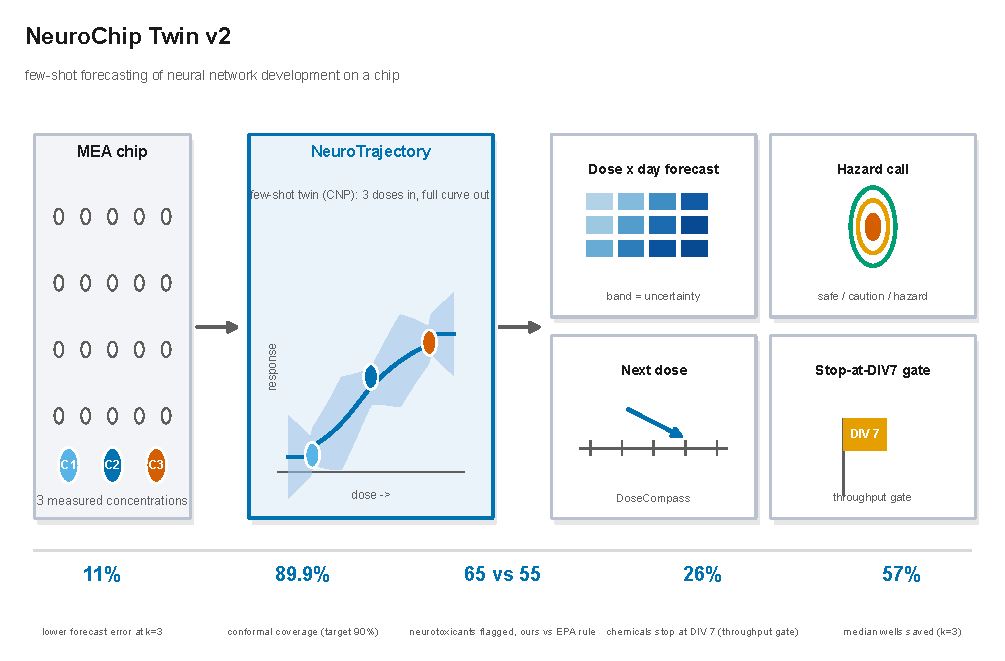
\includegraphics[width=0.94\linewidth]{figures/visuals/graphical_abstract.pdf}
\end{center}

% ------------------------------------------------------------------------------------------ summary (about 250 words)
\begin{summarybox}
{\sffamily\bfseries\color{accent}Summary.}\;
Every compound tested on a neural organ-on-a-chip or microelectrode-array (MEA) platform costs a full
dose--response campaign: typically seven concentrations, replicate wells and twelve days of culture, analysed one
endpoint at a time and forgotten by the next compound. NeuroChip Twin v2 learns from \nChem{} chemicals of the US
EPA network formation assay (rat cortical neurons, 17 network features at DIV 5, 7, 9 and 12). Given three
measured concentrations of a new chemical, it forecasts the whole dose\,\(\times\)\,day response with calibrated
uncertainty, calls its developmental-neurotoxicity hazard, proposes the next concentration and flags cultures
that can stop at DIV\,7. Every result is out of fold, against executed baselines and an exact reproduction of
EPA's hazard rules, and every number in this report is rendered from a versioned result file.
\end{summarybox}

\begin{table}[!ht]
\centering\footnotesize
\caption{Key numbers (unseen chemicals; 95\% CIs in \cref{tab:glance} and the Results).}\label{tab:keynumbers}
\begin{tabularx}{\linewidth}{@{}>{\raggedright\arraybackslash}p{3.3cm}X@{}}
\toprule
Forecast from three doses & \RtwoRel\% lower curve error than the best of five executed baselines (\RtwoFRel\% on four never-inspected folds) \\
Hazard call from three doses & 65 known neurotoxicants detected against 52--56 for EPA's rules on all concentrations (same 97 chemicals), with \wellsSaved\% fewer treated wells \\
Calibrated intervals & coverage \RsevCov{} for nominal 90\% intervals; abstained forecasts (\RsevAbst\%, close to the rate fixed by the threshold) are the least reliable ones \\
Stop at DIV\,7 & 26\% of chemicals stop after two of four recordings (throughput gate); the twin's safety gate lets 3 known neurotoxicants exit instead of 13 \\
Next dose & measuring the top concentration first raises activity detection from \RsixbFixAcc\% to \RsixbAcc\% \\
Next assay to add & full-range viability would cut forecast error by 8.3\% with one measured dose (scenario) \\
\bottomrule
\end{tabularx}
\end{table}

\paragraph{Innovation}
(1)~\emph{A chemical is a few-shot task.} One model, meta-learned across \nChem{} chemicals, forecasts the full
dose\,\(\times\)\,DIV development of all 17 network features for a chemical it has never seen (\cref{sec:r2}).
(2)~\emph{An interpolation-informed gated decoder with dose-local attention}, which learns per feature and day
how far to trust the measured neighbours; removing it costs
6.9\% accuracy at \(k=3\) (\cref{sec:r9}).
(3)~\emph{A toxicology-specific trust layer}: cross-conformal intervals stratified by cytotoxicity and number of
measured doses, with epistemic abstention (\cref{sec:r7}). (4)~\emph{A closed decision loop for the lab}: hazard
call, next concentration and a DIV\,7 exit gate, each validated on real wells under preregistered protocols
against exactly reproduced EPA rules (\cref{sec:r4,sec:r6,sec:r11}).

{\small\color{muted}\noindent\textit{Reading guide.} \Cref{tab:rubric} maps every section to the Kaggle and
Pazhou evaluation criteria. Evidence boundaries are stated in \cref{sec:boundaries}; tied and negative results,
which shaped the design, are in \cref{sec:r3,sec:r6,sec:r11,sec:r5,sec:darwin} and \appref{app:ownarch}.\par}

% ======================================================================================================
\section{Problem and users}\label{sec:problem}

\paragraph{The bottleneck}
Developmental neurotoxicity (DNT) testing is moving from animal studies to an in-vitro battery of new
approach methodologies~\cite{oecd2023dnt,masjosthusmann2020establishment,carstens2022integrating}. Its
functional anchor is the network formation assay (NFA): rat primary cortical neurons grow on 48-well MEA
plates while exposed to a chemical, and spontaneous activity is recorded as the network forms at days
in vitro (DIV) 5, 7, 9 and 12~\cite{brown2016evaluation,frank2017developmental,shafer2019evaluation}.
Every compound costs a full dose--response campaign: \nSevenLv{} of the \nChem{} chemicals in the public NFA
record were tested at seven concentrations, each in replicate wells followed to DIV\,12.
Compartmentalised neural chips, which impose directed axonal connectivity between
sub-networks~\cite{brewer2013toward,narula2017narrow,courte2023synapses}, raise the cost of each data point further.
Analysis is still descriptive: one concentration--response curve per endpoint and
day~\cite{sheffield2022tcplfit2,carstens2026current}, no calibrated uncertainty, and no use of the hundreds of
compounds already measured. The NFA readout, spontaneous network activity on an MEA, is the same functional
readout that compartmentalised neural chips use; the twin consumes any MEA recording mapped to its assay and chip
descriptors, as shown on a four-compartment chip (\cref{sec:r8}) and in the sponsor-data path of \cref{sec:value}.

\paragraph{Our question}
\emph{After measuring one to four concentrations of a new compound, can we forecast its full effect on
neural-network development---every feature, every day, every concentration---with calibrated uncertainty,
decide whether it is hazardous, and choose the next concentration to measure?} A model that answers this is a
digital twin in the sense the challenge sponsor describes, ``from experimental description toward predictive
simulation'': a data-driven simulator of network formation that can be queried at conditions that were never
run, and that is updated by every new experiment.

\paragraph{Users}
(i)~A neural organ-on-a-chip laboratory that runs compartmentalised chips instrumented for electrophysiology and
wants to spend its wells and chips on informative conditions, and to turn its recordings into a reusable,
predictive data asset. (ii)~Regulatory and pharmaceutical toxicologists running the DNT in-vitro battery, who
need hazard calls and potencies with honest uncertainty from fewer wells.

\paragraph{What the system delivers}
(1)~A provenance-tracked data asset (chemical\,\(\times\)\,dose\,\(\times\)\,DIV\,\(\times\)\,well\,\(\times\)\,feature)
with cohort and splits frozen by hash (\cref{sec:data}); (2)~\NT, a few-shot forecast of the 4\,\(\times\)\,17
developmental trajectory at any concentration for a chemical never seen in training (\cref{sec:method,sec:r2});
(3)~calibrated intervals with visible abstention (\cref{sec:r7}), a hazard call from three concentrations
(\cref{sec:r4}) and potency from the most reliable estimator we found (\cref{sec:r3}); (4)~\DC, the next
concentration to measure, validated retrospectively on real wells (\cref{sec:r6}); and (5)~a chip layer fitted on
axon-resolved recordings of a four-compartment hippocampal chip (\cref{sec:r8}).


% ======================================================================================================
\section{Data asset and compliance}\label{sec:data}

\Cref{tab:data} lists every data source. All are public and licensed for reuse; none contains personal or
clinical data. \Cref{fig:data} summarises the primary asset.

\begin{table}[t]
\centering\small
\caption{Data sources. Counts are those of the frozen cohort after identity resolution. \emph{Unpaired} means
that no well, plate or culture is shared with the NFA data.}\label{tab:data}
\begin{tabularx}{\linewidth}{@{}P{3.2cm}LP{3.0cm}P{2.6cm}@{}}
\toprule
Source & Content used & Role & Licence / terms \\
\midrule
EPA NFA~\cite{carstens2026current,shafer2019evaluation} &
rat cortical networks, 48-well MEA, DIV 5/7/9/12, 17 features; \nChem{} chemicals (\nSpid{} sample IDs),
\nRows{} well\,\(\times\)\,DIV records, \nPlates{} plates, \nLevels{} chemical\,\(\times\)\,concentration levels &
primary training and evaluation asset & US Government work; data only, analysis code not redistributed \\
EPA DNT reference labels~\cite{mundy2015expanding,mundy2024recommended} &
\nPos{} positive, \nNeg{} negative, \nUnl{} unlabelled chemicals in the cohort & hazard evaluation (R4, R5) & US Government work \\
EPA tcplfit2 NFA fits~\cite{sheffield2022tcplfit2,carstens2026current} &
published AUC and DIV12 endpoint fits for 241 chemicals &
independent potency reference (R3); EPA-rule reproduction (R4) & US Government work \\
PubChem / invitrodb~\cite{kim2023pubchem,feshuk2023toxcast} &
AlamarBlue (metabolic viability) and LDH (membrane damage) calls of the NFA (AIDs 2284083, 2284068), chemical level &
Mondrian strata (R7); R5 & US Government work \\
NTP DNT-DIVER~\cite{ntp2018integrative,behl2019screening} &
well-level viability for 64 cohort chemicals & viability-join audit & US Government work \\
Brewer 4-compartment MEA~\cite{lassers2023data,vakilna2021flow,lassers2023flow} &
EC\(\to\)DG\(\to\)CA3\(\to\)CA1\(\to\)EC sub-networks, \brTun{} single-axon tunnels per array; \brRec{} recordings,
\brAx{} sorted axons (\brFF{} feed-forward, \brFB{} feedback) & chip layer (R8) & CC0 1.0 \\
Harrill high-content imaging~\cite{harrill2018testing,harrill2019data} &
74 chemicals, 21 neurite, synapse and viability endpoints, 192 plates &
unpaired corroboration (X2) & US Government work \\
Kosnik acute MEA~\cite{kosnik2020concentration,kosnik2020data} &
384 samples on mature networks; literature truth set 41 neuroactive / 32 negative &
unpaired contrast (X3) & US Government work \\
\bottomrule
\end{tabularx}
\end{table}

\paragraph{Target representation}
For feature \(f\) of a well recorded on plate \(p\), date \(t\) and day \(d\), the raw value \(x\) is
variance-stabilised and expressed as an effect size in units of vehicle variability,
\begin{equation}\label{eq:target}
  g_f(x)=\operatorname{asinh}\!\big(x/c_f\big),\qquad
  y_{f,d}=\operatorname{clip}_{\pm 10}\!\left(\frac{g_f(x)-\operatorname{med}^{\,\mathrm{veh}}_{p,t,d}\,g_f}{s_{f,d}}\right),
\end{equation}
where \(c_f\) is a quarter of the pooled DIV\,12 vehicle median, the median runs over the vehicle wells of the
same plate, date and day, and \(s_{f,d}\) is the pooled within-plate robust standard deviation of vehicle
wells. All constants are fitted on vehicle wells only. Undefined values (for example burst duration in a well
without bursts) are masked, never imputed. Wells with a failed quality flag are excluded.

\paragraph{Frozen cohort and splits}
Before any model was fitted, the cohort, alias map, quality rules, normalisation and four split schemes were
frozen and hashed (freeze \file{G0}, \appref{app:hashes}). All sample IDs of a chemical, connected by DTXSID or
normalised name, fall in the same fold of the primary five-fold chemical split, stratified by DNT label. Distinct
substances are never merged (valproate and valproic acid, heptachlor and its epoxide are linked for leakage
checks but kept apart). Secondary splits by plate, by held-out dose level and by chemical family are frozen as
well; the results in this report use the primary chemical split only.

\paragraph{Compliance and licences}
EPA data are used as data; the EPA analysis repositories carry no licence file, so their code is cited, not
copied. Datasets with non-commercial terms were excluded (\appref{app:licences}). The R-data reader
\file{pyreadr} (AGPL-3.0) was replaced by \file{rdata} (MIT) with byte-identical output, recorded as freeze
amendment \file{G0-A001}. The code is released under the MIT licence.

\paragraph{What the feature layer is, and is not}
We intended to validate a clean-room re-implementation of the 17 NFA features against EPA's per-well values
(R1). The public spike archive shares 0 plates with the NFA record
(9 archive plates versus 163),
so fidelity is not estimable. The twin therefore models EPA's published features, and our feature engine is
applied to the Brewer chip only, as cross-platform analogues~\cite{cotterill2016characterization,ball2017multivariate}.

\begin{figure}[t]
\centering
\fig[0.94\linewidth]{figures/fig2_data.pdf}
\caption{The data asset. (a)~Tested concentrations per chemical and (b)~replicate wells per chemical
\(\times\) concentration in the EPA NFA cohort. (c)~Fraction of wells in which each feature is defined, by
DIV; burst and network-spike features are undefined in young networks and are masked, not imputed.
(d)~Layout of the Brewer four-compartment MEA: four sub-networks joined by single-axon tunnels with an
electrode at each end, which resolves the direction and conduction time of each axon.}\label{fig:data}
\end{figure}

\begin{figure}[!tbp]
\centering
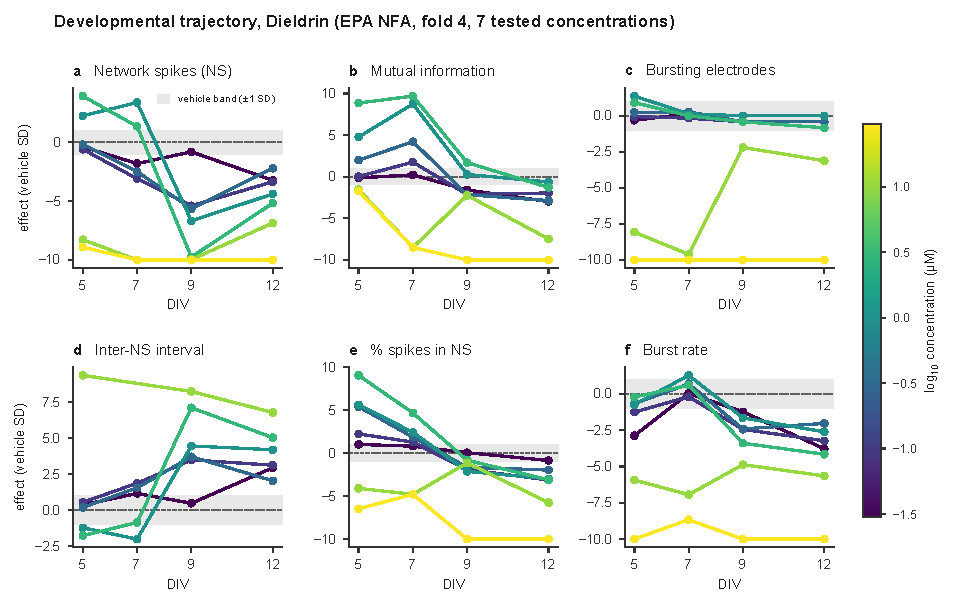
\includegraphics[width=0.92\linewidth,height=0.30\textheight,keepaspectratio]{figures/visuals/network_development.pdf}
\caption{What the primary data look like: measured development (DIV\,5--12) of six network features for dieldrin,
the reference-positive chemical with the largest measured effect in folds 1--4 (selection rule in
\file{make_visuals.py}); colour is concentration, grey is the vehicle band.}\label{fig:realdata}
\end{figure}

\begin{figure}[!tbp]
\centering
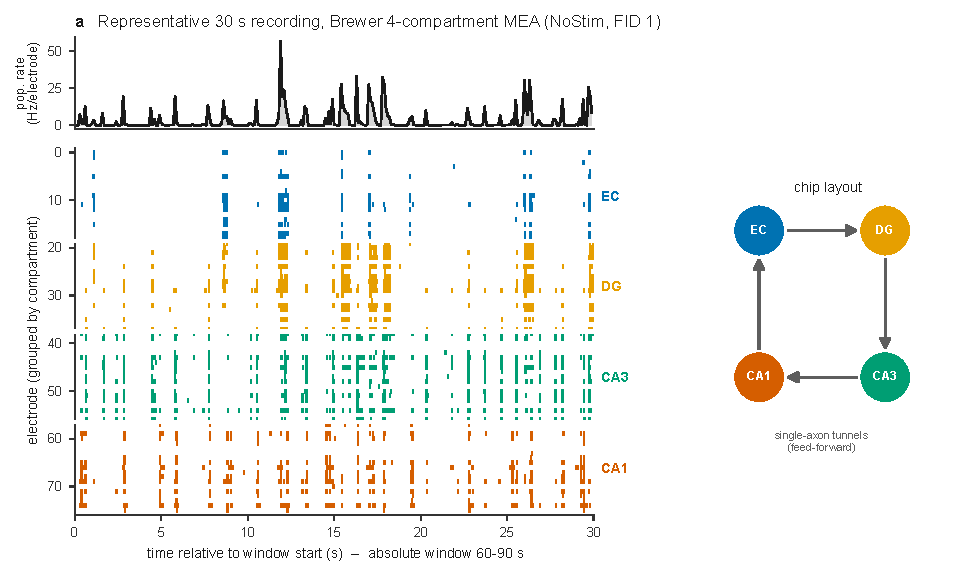
\includegraphics[width=0.92\linewidth,height=0.26\textheight,keepaspectratio]{figures/visuals/real_network_raster.pdf}
\caption{What the chip data look like: thirty seconds of spontaneous activity from an unstimulated four-compartment
Brewer chip, electrodes grouped by sub-network, with the population rate above and the directed tunnel ring
EC\(\to\)DG\(\to\)CA3\(\to\)CA1\(\to\)EC.}\label{fig:raster}
\end{figure}

% ======================================================================================================
\section{Method}\label{sec:method}

\subsection{Formulation: a chemical is a few-shot task}
For chemical \(c\), the wells form a set \(\mathcal{T}_c=\{(\ell_i,Y_i,M_i)\}_{i=1}^{n_c}\), where \(\ell_i\) is
the log\(_{10}\) concentration (\textmu M), \(Y_i\in\mathbb{R}^{4\times17}\) is the whole developmental
trajectory of well \(i\) in the units of \cref{eq:target}, and \(M_i\) its observation mask. \emph{Measuring}
\(k\) concentration levels reveals every replicate well at those levels, the context \(C_k\); the task is to
predict the wells at all other levels, and at any concentration in between, for a chemical never seen in
training. \(k=0\) asks for the population prior.

\subsection{NeuroTrajectory}
\NT{} (\cref{fig:system}) is a conditional neural process~\cite{garnelo2018conditional,garnelo2018neural} with
a dose-local attentive path~\cite{kim2019attentive,vaswani2017attention} and an interpolation-informed residual
decoder. Concentrations enter through Fourier features~\cite{tancik2020fourier},
\(e(\ell)=W_e\,[z,\sin(\omega z),\cos(\omega z)]\) with \(z=(\ell+0.5)/1.5\) and \(\omega_j=0.5\cdot 2^{j}\),
\(j=0,\dots,n_\omega-1\); fewer frequencies make the response smoother in dose. For a query concentration \(q\),
\begin{align}
  h_i &= \phi\big([\,e(\ell_i),\;Y_i\odot M_i,\;M_i\,]\big), &
  r_g &= \tfrac{1}{|C_k|}\textstyle\sum_{i\in C_k} h_i, &
  r_\ell(q) &= \operatorname{MHA}\big(W_q e(q),\,W_k e(\ell_i),\,h_i\big),\label{eq:encoder}\\
  (\delta,s,\gamma) &= \psi\big([\,r_g,\;r_\ell(q),\;e(q),\;W_I[I(q),\Delta(q)]\,]\big), &
  \mu(q) &= \sigma(\gamma)\odot I(q)+\delta, &
  \sigma(q) &= 0.02+\operatorname{softplus}(s),\label{eq:decoder}
\end{align}
where \(\phi,\psi\) are multilayer perceptrons, \(\operatorname{MHA}\) is multi-head attention whose keys are
the measured doses, \(I(q)\in\mathbb{R}^{4\times 17}\) is the piecewise-linear interpolation in log dose of the
context level means (flat outside the measured range), \(\Delta(q)\) is the distance to the nearest measured
level, and \(\sigma(\cdot)\) is the logistic gate. The gate lets the network decide, per feature and day, how
far to trust the measured neighbours and how much to correct them with what it has learned across chemicals.
With an empty context, \(r_g\) and \(r_\ell\) are learned vectors, \(I\equiv 0\), and the model returns its prior.

\paragraph{Meta-training}
Each episode samples a training chemical and a random number \(k\le 5\) of its levels as context, and scores the
masked negative log-likelihood of all its wells under a Gaussian or a Laplace likelihood,
\begin{equation}\label{eq:loss}
  \mathcal{L}=-\frac{1}{\sum M}\sum_{i,d,f} M_{i,d,f}\,\log p\big(y_{i,d,f}\mid\mu_{d,f}(\ell_i),\,\sigma_{d,f}(\ell_i)\big),
\end{equation}
with AdamW, a one-cycle schedule, 4000 steps and batches of 32 fixed a priori (PyTorch~\cite{paszke2019pytorch}).

\paragraph{Nested selection and ensemble}
Inside each outer training set, one inner fold chooses the likelihood (Gaussian or Laplace) and the decoder
(plain or interpolation-informed); outer test chemicals are never used for any choice. The interpolation-informed
decoder was selected in every outer fold. The chosen configuration is retrained with three seeds, and the
ensemble predicts
\(\bar\mu=\tfrac13\sum_m\mu_m\) with scale \(\bar\sigma^2=\tfrac13\sum_m\sigma_m^2+\operatorname{Var}_m(\mu_m)\).
A second grid (\file{v2}) adds the number of dose frequencies \(n_\omega\in\{ 3, 8 \}\) as a smoothness
hyperparameter; we report it as a robustness check.

\subsection{Calibration and abstention}
Every prediction used for calibration is out of fold. For a held-out well entry the nonconformity score is
\(s=|y-\bar\mu|/\bar\sigma\). In cross-conformal
fashion~\cite{vovk2015cross,vovk2022algorithmic,lei2018distribution,angelopoulos2023conformal}, the interval for
outer fold \(g\) and Mondrian stratum \(\pi\) (cytotoxicity regime \(\times\) number of measured levels \(k\)) is
\begin{equation}\label{eq:conformal}
  \bar\mu\pm\hat q_{g,\pi}\,\bar\sigma,\qquad
  \hat q_{g,\pi}=\text{the }\big\lceil (n+1)(1-\alpha)\big\rceil/n\text{ empirical quantile of }\{s:\ \text{fold}\neq g,\ \text{stratum}=\pi\}.
\end{equation}
The cytotoxicity regime is set at chemical level from the AlamarBlue and LDH calls of the NFA assay
(\emph{cytotoxic} if either is active, \emph{non-cytotoxic} if both are inactive, otherwise
\emph{indeterminate}); it is never a same-well viability readout. The twin abstains when the epistemic ratio
\(e=\overline{\operatorname{sd}_m(\mu_m)}/\overline{\bar\sigma}\) exceeds the 90th percentile of its values in
the calibration folds.

\subsection{Derived potency and hazard}\label{sec:potency-def}
The developmental summary of feature \(f\) is \(A_f(\ell)=\tfrac14\sum_{d}y_{f,d}(\ell)\), in vehicle standard
deviations. A chemical is active on \(f\) if \(|A_f|\) reaches the benchmark response \(\mathrm{BMR}=3\)
within the tested range; \(\mathrm{BMC}_f=\min\{\ell:|A_f(\ell)|\ge\mathrm{BMR}\}\) on a 120-point log grid, and
the chemical's potency is its most sensitive feature, \(\mathrm{BMC}=\min_f\mathrm{BMC}_f\). This BMC is a
threshold-crossing concentration on a grid, not a model-fitted benchmark dose (BMD/BMDL) such as those of EPA's
tcplfit2; comparisons with tcplfit2 potencies (R3) are rank and error comparisons, not equivalence. The hazard call is
an L2 logistic regression (balanced class weights, \(C=1\) fixed a priori) on 51 trajectory summaries---for each
feature, \(\max|A_f|\), \(A_f\) at the top concentration and \(\mathrm{BMC}_f\)---with out-of-fold
probabilities from the frozen chemical folds.

\subsection{DoseCompass: the next concentration by expected information}
Given the measured levels, \DC{} draws \(S=2000\) plausible
full-information data sets: measured levels keep their observed summaries, and every unmeasured level
\(\ell\) receives \(A_s(\ell)=\mu^{(m)}_A(\ell)+\tau\,\operatorname{sd}^{(m)}_A(\ell)\,\varepsilon_s(\ell)\),
where \(m\) cycles over ensemble members and \(\varepsilon_s\) is a Gaussian process in log dose with length
scale \(\ell_{\mathrm{GP}}\). Each sample yields a potency \(P_s\) (inactive, or the BMC in
0.25-log bins) and, for each candidate level \(u\), an outcome
\(O_s(u)\) (\(\max_f|A_s(u,f)|\) binned at 0.5,
1 and
2\,\(\times\)\,BMR). The next level maximises the expected
information gain~\cite{lindley1956measure,chaloner1995bayesian}
\begin{equation}\label{eq:eig}
  u^\star=\arg\max_u\ \mathrm{EIG}(u),\qquad \mathrm{EIG}(u)=I\big(P;O(u)\big)=\sum_{P,O}\hat p(P,O)\log_2\frac{\hat p(P,O)}{\hat p(P)\,\hat p(O)}.
\end{equation}
\((\tau,\ell_{\mathrm{GP}})\) are chosen per outer fold by cross-fitting the log score of the reference
potency bin on the other four folds only; the choice was
\((\tau,\ell_{\mathrm{GP}})=(0.5,\,1)\)
in every fold, inside the grid. The planner reads only wells at measured levels.

\subsection{ChipLayer: directed propagation on a four-compartment chip}
For each recording, the four sub-networks form a directed ring (EC\(\to\)DG\(\to\)CA3\(\to\)CA1\(\to\)EC is
feed-forward); each tunnel carries sorted axons with direction and conduction time~\cite{narula2017narrow,vakilna2021flow}.
An empirical-Bayes model shrinks the feed-forward fraction of a tunnel towards its anatomical pair and the pair
towards the global rate,
\begin{equation}\label{eq:chip}
  \hat p_{\mathrm{pair}}=\frac{n^{\mathrm{ff}}_{\mathrm{pair}}+\kappa\,\hat p_0}{n_{\mathrm{pair}}+\kappa},\qquad
  \hat p_{t}=\frac{n^{\mathrm{ff}}_{t}+\kappa\,\hat p_{\mathrm{pair}(t)}}{n_{t}+\kappa},\qquad \kappa=8\ \text{axons},
\end{equation}
with the same shrinkage for the discrete distribution of conduction times. Because the orientation of an array
changes which anatomical pair a physical tunnel joins, pairs are resolved per recording.

\subsection{Baselines and statistics}
Every method receives exactly the same measured wells: zero effect; the mean of the measured levels;
piecewise-linear interpolation in log dose; a Hill curve per endpoint (exhaustive search over AC50 and slope,
closed-form efficacy); and analog nearest-neighbour transfer from the training chemicals whose responses at the
measured concentrations are closest. The primary forecasting metric is the \emph{curve MAE}: the absolute
error against the mean of the replicate wells at each held-out level, averaged per chemical and then over
chemicals, over five seeded designs per \(k\). Differences are paired by chemical and bootstrapped over chemicals
(4000 resamples)~\cite{efron1993introduction}; proportions carry Clopper--Pearson intervals~\cite{clopper1934use};
paired classifiers are compared with the exact McNemar test~\cite{mcnemar1947note}.

\begin{figure}[t]
\centering
\fig{figures/fig1_system.pdf}
\caption{System overview. Public, licensed inputs are unified into a frozen, provenance-tracked asset.
\NT{} forecasts the dose\,\(\times\)\,DIV\,\(\times\)\,feature response of an unseen chemical from \(k\) measured
concentrations; calibration and abstention wrap every forecast; the decision layer returns a hazard call, a
potency and the next concentration to measure, closing the laboratory loop. The chip layer is fitted on
axon-resolved recordings of a four-compartment hippocampal chip and is descriptive (no cross-platform calibration).}\label{fig:system}
\end{figure}

% ======================================================================================================
\section{System and implementation}\label{sec:system}

The system is a Python package (\file{src/neurotwin}) with one module per layer and a script per result; each
script writes one JSON file in \file{results/}, and nothing else is a source of numbers (\cref{tab:modules}).

\begin{table}[t]
\centering\small
\caption{Modules, entry points and the result files they write.}\label{tab:modules}
\footnotesize
\begin{tabularx}{\linewidth}{@{}P{2.9cm}P{6.3cm}L@{}}
\toprule
Layer & Code (\file{src/neurotwin/}, \file{scripts/}) & Output (\file{results/}) \\
\midrule
Ingestion and freeze & \file{data/epa_nfa.py}, \file{data/cohort.py}, \file{data/brewer.py}, \file{data/harrill.py}, \file{data/kosnik.py} & \file{freeze_g0.json}, \file{cohort_freeze.json}, \file{splits_*.json}, \file{data_audit_brewer.json} \\
EPA-rule reproduction & \file{data/epa_nfa.py} (hit-count rules on EPA's published fits) & \file{epa_baseline_repro.json} \\
Forecasting (\NT) & \file{models/cnp.py}, \file{models/trajectory.py}, \file{scripts/run_trajectory_cv.py} & \file{trajectory_cv.json}, \file{trajectory_cv_v2.json} \\
Calibration, abstention & \file{scripts/run_conformal.py} & \file{conformal_r7.json} \\
Potency and hazard & \file{models/potency.py}, \file{scripts/run_potency.py}, \file{scripts/run_dnt_r4.py} & \file{potency_r3.json}, \file{potency_r3b.json}, \file{dnt_r4.json} \\
Planning (\DC) & \file{planner/eig.py}, \file{scripts/run_dosecompass*.py} & \file{r6_dosecompass.json}, \file{r6b_dosecompass_anchored.json} \\
Chip layer & \file{chip/propagation.py}, \file{features/mea.py}, \file{scripts/run_chiplayer.py} & \file{r8_chiplayer.json}, \file{chiplayer_params.json}, \file{brewer_features.json} \\
Cross-assay, diagnostics & \file{scripts/run_crossassay.py}, \file{run_ablations.py}, \file{run_selectivity_failures.py} & \file{x2_harrill.json}, \file{x3_kosnik.json}, \file{r9_ablations.json}, \file{r10_failures.json}, \file{r5_selectivity.json} \\
\bottomrule
\end{tabularx}
\end{table}

\paragraph{Delivery}
Four entry points share one compute core and the cross-validated weights shipped in the data bundle. The
command-line demo runs on a laptop CPU without network access, loads the models of the fold that never saw the
chosen chemical, forecasts its trajectory from \(k\) measured concentrations and then reveals the held-out
wells and scores the forecast against the same baselines; a Gradio app exposes the same core interactively; a
static explorer (GitHub Pages) serves precomputed held-out forecasts for every chemical; and a Kaggle notebook
reproduces the headline tables. Training ran on a single consumer GPU; inference, the demo and the tests run on
CPU.

\paragraph{Credibility layer}
\file{scripts/render_docs.py} fills every number of this report, the README and the Writeup from
\file{results/*.json}, stops when a token does not resolve, and writes a ledger of each value with its source;
\file{scripts/check_numbers.py} fails continuous integration when a rendered document (this report, its figure
captions, the README) contains an untraced number, or when a template contains a typed number that is not a
structural constant justified in \file{docs/number_allowlist.txt}; \file{scripts/check_freeze_g0.py} verifies
every frozen file against its hash.

% ======================================================================================================
\section{Results}\label{sec:results}

All results are out of fold under the frozen chemical split: a chemical is only ever scored by models that
never saw it. \Cref{tab:glance} summarises them; each subsection states the protocol and our reading of the
evidence, negative results included.

\begin{table}[t]
\centering\small
\caption{Results at a glance (primary analyses; 95\% confidence intervals in brackets).}\label{tab:glance}
\begin{tabularx}{\linewidth}{@{}P{0.8cm}P{4.2cm}LP{1.5cm}@{}}
\toprule
ID & Question & Result & Verdict \\
\midrule
R2 & Forecast unseen chemicals from \(k=3\) doses? & curve MAE \RtwoNT{} vs \RtwoBase{} (best baseline); \sgn{\RtwoDiff}\ \RtwoCI; folds 1--4: \RtwoFRel\% lower & \vpos \\
R7 & Are 90\% intervals calibrated? & coverage \RsevCov{} \RsevCI{} after conformal (\RsevPar{} before); abstention \RsevAbst\% & \vpos \\
R4 & Hazard call from three doses? & BA \RfourBA\% vs \RfourEpaLo--\RfourEpaHi\% (EPA rules, same \RfourN{} chemicals); McNemar significant in one of three & \vmod \\
R3 & Potency from the model? & model-derived BMC worse than interpolation of measured doses at every \(k\) & \vneg \\
R6 & Choose the next dose? & ties log-spaced (\sgn{ -0.006 } \ci{ -0.060 }{ 0.053 }); \RsixRandRel\% better than random & \vtie \\
R8 & Directed chip connectivity? & feed-forward fraction MAE \sgn{ -0.036 } vs tunnel means; conduction: no gain & \vmod \\
X2 & Network vs morphology? & NFA active in 96\% of morphology-active chemicals; network BMC lower by 0.56 log\(_{10}\) & \vpos \\
X3 & Developmental vs acute? & activity BA 65.4\%; potency ranks do not transfer & \vmod \\
R9 & Do the components matter? & removing the interpolation-informed decoder: +6.9\% error at \(k=3\) & \vpos \\
R5 & Specific vs cytotoxic disruption? & selectivity index AUROC 0.51, no better than chance & \vneg \\
\bottomrule
\end{tabularx}
\end{table}

% ------------------------------------------------------------------------------------------ R2
\subsection{R2 --- Forecasting network formation in unseen chemicals}\label{sec:r2}

\paragraph{Protocol}
Five outer folds of \nChem{} chemicals; for each held-out chemical and \(k\in\{0,\dots,4\}\), five seeded designs
choose the measured levels; all other levels are targets. One short development smoke run (one seed) was
evaluated on outer fold 0 and motivated adding the interpolation-informed decoder as a candidate; the final choice
is nested, and we report folds 1--4 (\nFoldsOneFour{} chemicals, never inspected) separately.

\begin{table}[t]
\centering\footnotesize
\caption{R2: curve MAE (vehicle SD units; lower is better) for held-out chemicals, all five folds. \(\Delta\) is
\NT{} minus the best baseline at that \(k\) (marked \(^\dagger\)), paired over chemicals.}\label{tab:r2}
\setlength{\tabcolsep}{3.6pt}
\begin{tabular}{@{}c cccccc c r r@{}}
\toprule
\(k\) & \NT & Interp. & Hill & Analog kNN & Ctx.\ mean & Zero & \(\Delta\) vs best [95\% CI] & \(\Delta\)\% all & \(\Delta\)\% folds 1--4 \\
\midrule
0 & \textbf{ 1.689 } & 1.769 & 1.769 & 1.702\(^\dagger\) & 1.769 & 1.769 & \sgn{ -0.013 } \ci{ -0.027 }{ 0.000 } & \sgn{ -0.8 } & \sgn{ -0.4 } \\
1 & \textbf{ 1.415 } & 1.875 & 1.875 & 1.494\(^\dagger\) & 1.875 & 1.770 & \sgn{ -0.080 } \ci{ -0.115 }{ -0.040 } & \sgn{ -5.3 } & \sgn{ -5.8 } \\
2 & \textbf{ 1.279 } & 1.533 & 1.533 & 1.393\(^\dagger\) & 1.697 & 1.773 & \sgn{ -0.114 } \ci{ -0.147 }{ -0.078 } & \sgn{ -8.2 } & \sgn{ -8.8 } \\
3 & \textbf{ 1.180 } & 1.325\(^\dagger\) & 1.435 & 1.327 & 1.607 & 1.783 & \sgn{ -0.145 } \ci{ -0.188 }{ -0.099 } & \sgn{ -11.0 } & \sgn{ -11.2 } \\
4 & \textbf{ 1.138 } & 1.239\(^\dagger\) & 1.308 & 1.311 & 1.590 & 1.810 & \sgn{ -0.100 } \ci{ -0.136 }{ -0.061 } & \sgn{ -8.1 } & \sgn{ -8.8 } \\
\bottomrule
\end{tabular}
\end{table}

\paragraph{Result}
\NT{} has the lowest error at every \(k\) (\cref{tab:r2,fig:forecast}). With three measured concentrations
its curve MAE is \RtwoNT{} against \RtwoBase{} for log-linear interpolation, the best baseline: a paired
difference of \sgn{\RtwoDiff}\ \RtwoCI, \RtwoRel\% lower error, and a gain for \RtwoImp\% of chemicals. On the
four never-inspected folds the gain is \RtwoFRel\% (paired difference \RtwoFCI), for \RtwoFImp\% of chemicals. The advantage grows
from one to three measured concentrations and is still clear at four; with no measurement (\(k=0\)) the learned
prior only ties the analog baseline. Against a Hill curve per endpoint, the usual practice, the error falls by
17.8\% at \(k=3\).
The same ranking holds for the noisier well-level error
(\sgn{ -0.121 }
\ci{ -0.148 }{ -0.092 }
against analog kNN at \(k=3\)). The \file{v2} grid, which also tunes dose smoothness, gives
1.181 at \(k=3\)
(10.9\% below the best baseline;
11.2\% on folds 1--4): the result
does not hinge on that hyperparameter.

\paragraph{Reading}
Meta-learning across chemicals transfers: a new compound's trajectory is predicted better by a model that has
seen how \nChem{} others perturb network formation than by any per-chemical fit of the same wells. The gain is
largest where interpolation is weakest---between and beyond the measured doses, and in features whose response
is not monotone in dose (\cref{fig:examples}). \Cref{sec:r10} shows where the model loses.

\begin{figure}[t]
\centering
\fig{figures/fig3_forecast_main.pdf}
\caption{R2 forecasting. (a)~Curve MAE of held-out chemicals against the number of measured concentrations \(k\),
with chemical-bootstrap 95\% intervals. (b)~Paired difference to the best baseline at each \(k\) for all folds,
for folds 1--4 (never inspected during development) and for the \file{v2} grid with tuned dose smoothness.
(c)~Per-chemical error at \(k=3\) on folds 1--4; points below the diagonal are chemicals where \NT{} is better.}\label{fig:forecast}
\end{figure}

\begin{figure}[t]
\centering
\fig[0.80\linewidth]{figures/fig4_examples.pdf}
\caption{Held-out forecasts at \(k=3\) for three chemicals chosen by a fixed rule: the 90th, 50th and 10th
percentiles of the per-chemical gain over interpolation (Heptachlor epoxide B, DDT,
Retinoic acid; all reference positives), each with its median design, never its worst; rows are three
fixed features. Black: wells shown to the model; open: held-out wells, revealed after forecasting. Blue: \NT{}
mean with its pooled conformal 90\% band; dashed: log-linear interpolation of the measured levels.}\label{fig:examples}
\end{figure}

% ------------------------------------------------------------------------------------------ R7
\subsection{R7 --- Calibrated uncertainty and abstention}\label{sec:r7}

\paragraph{Protocol}
Cross-conformal Mondrian calibration (\cref{eq:conformal}) over the \nChem{} out-of-fold chemicals
(\nNonCyto{} non-cytotoxic, \nCyto{} cytotoxic, \nIndet{} indeterminate), for \(k=1,2,3\) and nominal 80, 90 and
95\% intervals. Coverage is the mean over held-out chemicals, with a chemical-bootstrap interval.

\begin{table}[t]
\centering\footnotesize
\caption{R7: observed coverage of nominal 90\% intervals on held-out wells, before (parametric ensemble) and
after cross-conformal calibration, with mean interval width (vehicle SD units) and coverage per Mondrian stratum.}\label{tab:r7}
\begin{tabular}{@{}c cc cc ccc@{}}
\toprule
& \multicolumn{2}{c}{Coverage (nominal 0.90)} & \multicolumn{2}{c}{Mean width} & \multicolumn{3}{c}{Conformal coverage by regime} \\
\cmidrule(lr){2-3}\cmidrule(lr){4-5}\cmidrule(l){6-8}
\(k\) & parametric & conformal [95\% CI] & param. & conf. & non-cytotoxic & cytotoxic & indeterminate \\
\midrule
1 & 0.869 & 0.898 \ci{ 0.890 }{ 0.906 } & 7.26 & 8.32 & 0.899 & 0.896 & 0.903 \\
2 & 0.875 & 0.899 \ci{ 0.891 }{ 0.907 } & 6.95 & 7.83 & 0.897 & 0.900 & 0.907 \\
3 & 0.882 & 0.899 \ci{ 0.891 }{ 0.906 } & 6.77 & 7.41 & 0.897 & 0.900 & 0.904 \\
\bottomrule
\end{tabular}
\end{table}

\paragraph{Result}
The ensemble's own intervals are slightly too narrow (\RsevPar{} coverage at \(k=3\) for a nominal 0.90).
After calibration, coverage is \RsevCov{} \RsevCI{} and is on target at every \(k\), in every stratum and at every
level: at \(k=3\), 0.800 for nominal 0.80 and
0.949 for nominal 0.95 (\cref{tab:r7,fig:calibration}).
Calibration has a price that is itself informative: intervals are wider for cytotoxic than for non-cytotoxic
chemicals (8.05 vs
6.66 vehicle SD at \(k=3\); indeterminate
chemicals are as wide), because network responses there collapse abruptly, and all intervals narrow as doses are added. The abstention rule flags
\RsevAbst\% of forecasts; their curve MAE is 1.666, against
1.250 for retained forecasts, and the abstention rate falls from
14.4\% at \(k=1\) to 7.8\% at \(k=3\).

\paragraph{Reading}
Coverage is a measured property inside the calibration domain (rat cortical NFA, chemical-level exchangeability),
not a guarantee that transfers to other species, cell sources or chips. Within that domain, a user can read a
twin interval at face value and can see when the twin declines to answer.

\begin{figure}[t]
\centering
\fig[0.86\linewidth]{figures/fig5_calibration.pdf}
\caption{R7 calibration. (a)~Observed minus nominal coverage of held-out wells, before (open) and after (filled)
cross-conformal calibration, for \(k=1,2,3\). (b)~Conformal coverage per Mondrian stratum at 90\% nominal.
(c)~Mean width of 90\% intervals: the price of calibration is paid in cytotoxic and indeterminate chemicals. (d)~Curve MAE of
retained and abstained forecasts.}\label{fig:calibration}
\end{figure}

% ------------------------------------------------------------------------------------------ R4
\subsection{R4 --- A hazard call from three concentrations}\label{sec:r4}

\paragraph{Protocol}
Reference chemicals: the intersection of the EPA reference table with the cohort (\nPos{} positive, \nNeg{}
negative). Two variants were declared before evaluation: \emph{few-shot} (\(k=3\)), whose 51 summaries come
from the \NT{} forecast given three spread concentrations, and \emph{all doses}, from the measured levels.
Comparators are EPA's published hit-count rules (DIV12, AUC\,3-hit, Top-2), which we reproduce exactly on EPA's
own cohort: 86 positive and 19
negative chemicals, a difference of 0.0
percentage points on every selected published metric, and zero mismatches in the per-chemical hit sums. The
comparison is paired on the \RfourN{} chemicals with a per-chemical EPA call. Two caveats are ours to state:
EPA's endpoint fits are taken as published, not refitted from wells, and its Top-\(k\) features were ranked on
the full reference set (in sample), so its published balanced accuracy is not an out-of-sample ceiling.

\begin{table}[t]
\centering\footnotesize
\caption{R4: hazard calls on the same \RfourN{} reference chemicals (Clopper--Pearson 95\% intervals). McNemar
columns compare the pre-specified few-shot variant with each EPA rule: chemicals only we call correctly, only
the rule calls correctly, and the exact two-sided \(p\).}\label{tab:r4}
\begin{tabular}{@{}l ll c cc c@{}}
\toprule
Method & Sensitivity (\%) & Specificity (\%) & BA (\%) & ours only & rule only & \(p\) \\
\midrule
\NT{}, \(k=3\) (pre-specified) & 83.3 \ci{ 73.2 }{ 90.8 } & 89.5 \ci{ 66.9 }{ 98.7 } & \textbf{ 86.4 } & & & \\
\NT{}, all doses & 80.8 \ci{ 70.3 }{ 88.8 } & 68.4 \ci{ 43.5 }{ 87.4 } & 74.6 & & & \\
\midrule
EPA rule DIV12 & 70.5 \ci{ 59.1 }{ 80.3 } & 94.7 \ci{ 74.0 }{ 99.9 } & 82.6 & 14 & 5 & 0.064 \\
EPA rule AUC\,3-hit & 66.7 \ci{ 55.1 }{ 76.9 } & 100.0 \ci{ 82.3 }{ 100.0 } & 83.3 & 14 & 3 & 0.013 \\
EPA rule Top-2 & 71.8 \ci{ 60.5 }{ 81.4 } & 100.0 \ci{ 82.3 }{ 100.0 } & 85.9 & 11 & 4 & 0.118 \\
\bottomrule
\end{tabular}
\end{table}

\begin{figure}[t]
\centering
\fig{figures/fig6_hazard.pdf}
\caption{R4 hazard call and R3 potency. (a)~Sensitivity and specificity with Clopper--Pearson 95\% intervals on the
same \RfourN{} reference chemicals, for \NT{} (\(k=3\), pre-specified; and all doses) and the reproduced EPA
rules. (b)~Discordant chemicals between the \(k=3\) call and each EPA rule, with the exact McNemar \(p\).
(c)~R3/R3b potency: paired difference in composite error to interpolation of the measured doses (above zero,
interpolation is better; this is why BMC is reported by interpolation).}\label{fig:hazard}
\end{figure}

\paragraph{Result}
On the \RfourN{} chemicals with a per-chemical EPA call, three concentrations completed by the twin detect
65 known neurotoxicants, against 52--56
for EPA's rules on the full series, at the cost of 2 false alarms among the
negatives (EPA: 0--1); balanced accuracy is
\RfourBA\% (\cref{tab:r4,fig:hazard}). On all \nPos{}\,+\,\nNeg{} reference chemicals the AUROC is
0.915
\ci{ 0.853 }{ 0.965 }. Against AUC\,3-hit, it calls 14
chemicals correctly that the rule misses and misses 3
that the rule gets right (\(p=\RfourP\)); against DIV12 and Top-2 the differences are not significant. The
all-doses variant is weaker (balanced accuracy 74.6\%,
McNemar \(p\ge0.36\) against every rule).

\paragraph{Reading}
For a screening tier, the higher sensitivity is the more useful operating point: three concentrations,
completed by the twin, carry at least as much hazard information as EPA's rules applied to the full series.
Cytotoxicity does not explain the result: most reference positives are cytotoxic and almost no negatives are
(\cref{sec:r5}), but among the 53 non-cytotoxic chemicals (a secondary, post-hoc
stratification) the twin's balanced accuracy is 78.7\%, against
66.2--72.1\% for
EPA's rules, with lower sensitivity for every method. We do not claim superiority: with \nNeg{} negatives a specificity difference of one or two
chemicals moves balanced accuracy by several points, only one of three pre-declared comparisons reaches
\(p<0.05\), and EPA's Top-\(k\) rules had an in-sample advantage. That the few-shot variant beats the all-doses
variant is consistent with the forecast acting as a learned denoiser of replicate noise; we report it and do not
build on it.

% ------------------------------------------------------------------------------------------ R3
\subsection{R3 and R3b --- Potency: a negative result that set a design decision}\label{sec:r3}

\paragraph{Protocol}
Potency (\cref{sec:potency-def}) recovered from \(k=2,3,4\) measured concentrations of the half of each chemical's
wells shown to the methods, scored against two independent references: EPA's published tcplfit2 fits (activity
agreement, and Spearman correlation of potencies for chemicals active in both), and a replicate-split reference
computed from the other half of the wells at all levels, so that no noise is shared. The per-chemical composite
error is \(|\Delta\mathrm{BMC}|\) (log\(_{10}\)) if active in both, 1 on activity disagreement and 0 if both are
inactive. R3b, registered in the decision log before it was run, completes the measured series with the forecast
only at the tested but unmeasured levels.

\begin{table}[t]
\centering\footnotesize
\caption{R3/R3b: potency error against the replicate-split reference (composite error, lower is better) and rank
agreement with EPA tcplfit2 potencies at \(k=3\). The last column is the paired difference to log-linear
interpolation at \(k=3\) (positive = worse than interpolation).}\label{tab:r3}
\begin{tabular}{@{}l ccc c c@{}}
\toprule
& \multicolumn{3}{c}{Composite error, replicate split} & Spearman vs EPA & \(\Delta\) vs interp., \(k=3\) \\
\cmidrule(lr){2-4}
Estimator & \(k=2\) & \(k=3\) & \(k=4\) & \(k=3\) & [95\% CI] \\
\midrule
\NT{}, dense grid (R3) & 0.960 & 0.967 & 0.920 & 0.65 & \sgn{ 0.106 } \ci{ 0.050 }{ 0.163 } \\
\NT{}, completed series (R3b) & 0.961 & 0.930 & 0.898 & 0.66 & \sgn{ 0.069 } \ci{ 0.026 }{ 0.111 } \\
Log-linear interpolation & 0.884 & \textbf{ 0.861 } & \textbf{ 0.847 } & 0.71 & --- \\
Hill per endpoint & 0.884 & 0.898 & 0.857 & \textbf{ 0.78 } & \\
Analog kNN & 1.039 & 0.968 & 0.946 & 0.74 & \\
\bottomrule
\end{tabular}
\end{table}

\paragraph{Result}
Potency read from the model's dense-grid forecast is worse than interpolation of the measured doses at every
\(k\): by 8.7,
12.3 and
8.6\% in composite error for \(k=2,3,4\),
with intervals that exclude zero (\cref{tab:r3}, \cref{fig:hazard}c). The registered R3b estimator improves on the dense grid at
\(k=3\) (\sgn{ -0.0365 }
\ci{ -0.0744 }{ -0.0002 })
and has the best activity agreement with the replicate reference (Cohen's \(\kappa\) of
0.27 versus
0.21), but it still loses to
interpolation in composite error. Against EPA's fits, a Hill curve per endpoint ranks potencies best at \(k=3\).
For scale, our potency rule applied to all tested levels agrees with EPA's activity calls with \(\kappa=\)
0.67 and ranks potencies with Spearman
0.75.

\paragraph{Reading and decision}
A benchmark crossing is a threshold event; small ripples of a smooth forecast between tested concentrations
create spurious early crossings, while interpolation cannot cross between two sub-threshold measurements. We
therefore \emph{report BMC by interpolation of measured doses} and use the twin for what it does well---the
trajectory, its uncertainty and the hazard call. A first version of this protocol (kept as
\file{potency_r3_v1_superseded_biased_reference.json}) used as reference the interpolation of all level means,
which coincides with the interpolation estimator at the measured levels and therefore favoured it (under that
reference the model appeared 26.2\% worse than
interpolation at \(k=3\)). It was replaced by the two independent references above; the gap shrank, but the
conclusion did not change.

% ------------------------------------------------------------------------------------------ R6 / R6b
\subsection{R6 and R6b --- Choosing the next concentration}\label{sec:r6}

\paragraph{Protocol}
Retrospective and preregistered (protocol SHA-256 in \appref{app:hashes}): with a budget of \(B=3\) levels, every
strategy starts from the same first level---the median tested concentration in R6 and the highest in R6b---and
adds \(B-1\) levels. \DC{} is compared with fixed log-spaced designs (primary), with 200 seeded random orders and
with an oracle subset that uses the hidden wells (an upper bound, not a strategy). Potency is then estimated
from the chosen levels by \NT{}; the metric is the composite error of R3 against the full-information
reference. R6b, the second protocol, was motivated by R6 (omitting the top concentration cost activity
detection); both are reported, without multiplicity correction.

\begin{table}[t]
\centering\footnotesize
\caption{R6/R6b at \(B=3\) (\NT{} estimator). Composite error (lower is better), activity accuracy and median
\(|\Delta\mathrm{BMC}|\) among chemicals active in both; \(\Delta\) is \DC{} minus the comparator, paired over
the \nChem{} chemicals.}\label{tab:r6}
\begin{tabular}{@{}l l c c c l@{}}
\toprule
Protocol & Strategy & Composite & Activity acc. & Med.\ \(|\Delta\)BMC\(|\) & \(\Delta\) [95\% CI] \\
\midrule
\multirow{5}{*}{\makecell[l]{R6\\(median first)}} & \DC & 0.445 & 0.840 & 0.221 & \\
& fixed log-spaced & 0.451 & 0.881 & 0.287 & \sgn{ -0.006 } \ci{ -0.060 }{ 0.053 } \\
& random (mean of 200) & 0.489 & 0.840 & 0.260 & \sgn{ -0.045 } \ci{ -0.088 }{ -0.002 } \\
& \DC, DIV 5--9 only & 0.444 & 0.852 & 0.244 & \\
& oracle (upper bound) & 0.147 & 0.947 & 0.037 & \\
\midrule
\multirow{3}{*}{\makecell[l]{R6b\\(top first)}} & \DC{}, anchored & 0.432 & 0.909 & 0.323 & \\
& fixed log-spaced & 0.451 & 0.881 & 0.287 & \sgn{ -0.019 } \ci{ -0.073 }{ 0.033 } \\
& random, anchored & 0.456 & 0.900 & 0.297 & \sgn{ -0.024 } \ci{ -0.065 }{ 0.013 } \\
\bottomrule
\end{tabular}
\end{table}

\paragraph{Result}
On the primary endpoint \DC{} ties fixed log-spaced designs in both protocols (\cref{tab:r6,fig:dosecompass}). It
beats random selection by \RsixRandRel\% in R6, with an interval that just excludes zero, and not significantly
in R6b. Anchoring on the top concentration raises activity detection: in R6b, \DC{} calls activity correctly for
\RsixbAcc\% of chemicals (\(\kappa=0.76\))
against \RsixbFixAcc\% (\(\kappa=0.68\))
for log-spaced designs, and it cuts the composite error on reference-inactive chemicals from
0.250 to
0.183.
The planner's belief is informative: after three levels its probability of activity has a Brier score of
0.104, against
0.186 for the base rate.
Deciding with DIV 5--9 only, before the last recording, loses nothing (\sgn{ -0.001 }
\ci{ -0.044 }{ 0.045 }).

\paragraph{Reading}
On EPA's grid of pre-chosen concentrations (seven for most chemicals), a good fixed design is hard to beat, and the large gap to the
oracle is mostly irreducible without seeing the wells. The operational lessons are concrete: measure the top
concentration first, then let the planner place the remaining budget, and decide before DIV\,12 if time matters.
A prospective trial with a free choice of concentrations is where the planner can show more (\cref{sec:value}).

\begin{figure}[t]
\centering
\fig[0.88\linewidth]{figures/fig7_dosecompass.pdf}
\caption{R6/R6b \DC. (a)~Twin posterior of the maximal developmental effect after one measurement of a
reference-positive chemical, and the expected information gain of each candidate level. (b)~Composite potency
error against the budget \(B\) for each strategy, with the 2.5--97.5\% band of 200 random orders. (c)~Paired
differences at \(B=3\) in the two registered protocols. (d)~Activity detection at \(B=3\).}\label{fig:dosecompass}
\end{figure}

% ------------------------------------------------------------------------------------------ R11
\subsection{R11 --- Early exit: stop the culture at DIV\,7}\label{sec:r11}

\paragraph{Protocol}
A neural culture takes twelve days and four recordings. R11 asks whether the first two recordings
(DIV\,5 and 7) are enough to decide which chemicals the complete assay would call inactive, so that their culture and
recordings can stop early while (almost) every active chemical continues. The idea comes from the team
lead's early-rejection filter for hardware pipelines, which discards work items from an early partial
signal before full processing \autocite{angulo2026silicon}. Here it is tested on biology with a preregistered
protocol (\appref{app:hashes}). The cohort is the 194 unseen chemicals of
folds 1--4. The reference is the fixed activity rule of \cref{sec:potency-def} applied to all DIVs and
concentrations, which gives 146 active and
48 inactive chemicals. Four scores see DIV\,5/7 only: \NT{} with
DIV\,9/12 masked, the same forecast with its upper 90\% band, the rule applied to the early data, and
persistence (DIV\,7 carried forward). For each fold, the exit threshold keeps 95\% of the active chemicals of
the other three folds. The primary endpoint is the fraction of inactive chemicals that exit.

\begin{table}[t]
\centering\footnotesize
\caption{R11 early exit from DIV\,5/7 (nested 95\%-sensitivity thresholds, \(n=194\)).
Sensitivity = active chemicals that continue to DIV\,12; exit = inactive chemicals stopped at DIV\,7; Clopper--Pearson
95\% CIs; AUROC with chemical bootstrap CI.}\label{tab:r11}
\begin{tabular}{@{}l c c c@{}}
\toprule
Score (DIV\,5/7 only) & Sensitivity [95\% CI] & Inactive exit [95\% CI] & AUROC [95\% CI] \\
\midrule
\NT{} (DIV\,9/12 masked) & 0.945 \ci{ 0.89 }{ 0.98 } & 0.458 \ci{ 0.31 }{ 0.61 } & 0.897 \ci{ 0.85 }{ 0.94 } \\
\NT{}, upper 90\% band & 0.938 \ci{ 0.89 }{ 0.97 } & 0.417 \ci{ 0.28 }{ 0.57 } & 0.833 \ci{ 0.76 }{ 0.89 } \\
Rule on DIV\,5/7 data & 0.945 \ci{ 0.89 }{ 0.98 } & 0.500 \ci{ 0.35 }{ 0.65 } & 0.920 \ci{ 0.88 }{ 0.95 } \\
Persistence (DIV\,7 carried forward) & 0.952 \ci{ 0.90 }{ 0.98 } & 0.917 \ci{ 0.80 }{ 0.98 } & 0.987 \ci{ 0.97 }{ 1.00 } \\
\bottomrule
\end{tabular}
\end{table}

\paragraph{Result}
Early exit works, and it has two operating points (\cref{tab:r11}). Against the assay's own rule, persistence
is the most efficient gate: it stops
92\% of the inactive chemicals at
DIV\,7 while 95\% of the active ones continue.
\NT{}, trained only with full-trajectory contexts, stops
46\% (difference
\sgn{ -0.46 }
\ci{ -0.62 }{ -0.30 }). By the
preregistered rule, persistence is the recommended throughput gate. An independent verifier recomputed every
score. The reference shares the DIV\,5/7 wells with every score, so R11b also evaluates every
method against a reference built from DIV\,9/12 only.
The external EPA DNT labels reverse the ranking where it matters most for safety: persistence would stop
13 of 63 known neurotoxicants at DIV\,7, the twin's upper 90\% band
3 (11 against 1 discordant chemicals,
exact McNemar \(p=0.006\); a secondary, post-hoc test), while both stop a similar number of
the 15 negatives (8 and 7). The system therefore
offers two gates: persistence for throughput, and the twin's upper band when a missed neurotoxicant is the
costlier error (15\% of chemicals stop).

\paragraph{Reading}
Most of the signal the complete assay will show is already present at DIV\,7, which makes an early-exit step
practical for a neural-OoC screening lab: with persistence,
26\% of all chemicals stop after two of
the four recordings. The circularity control and the external labels below qualify the choice of gate. The
primary twin was never trained to extrapolate in time, which explains its lower efficiency.

\paragraph{R11b --- retraining the twin to extrapolate in time}
A second protocol, registered after R11 and before any training, changed one thing: during training, the
context wells lose DIV\,9/12 with probability one half, while the targets stay complete. Retraining raised the
twin's inactive exit rate to 69\%
(AUROC 0.955; paired gain over v1
\sgn{ 0.23 }
\ci{ 0.07 }{ 0.39 }),
still below persistence
(\sgn{ -0.23 }
\ci{ -0.36 }{ -0.10 }).
Against the circularity control, a reference built from DIV\,9/12 only
(40 inactive chemicals), every early score
loses ground and persistence still leads: it stops
48\% of
the inactive chemicals against
25\% for the
retrained twin, whose gain over v1 disappears there
(\sgn{ -0.10 }
\ci{ -0.26 }{ 0.05 }).
Retraining did not harm dose interpolation (\(k=3\) curve MAE
\sgn{ -0.4 }\%,
\ci{ -1.3 }{ 0.5 }\%),
so the primary model remains the delivered forecaster. For a screening lab the recommendation is an auditable
gate at DIV\,7: persistence (the DIV\,7 network carried forward stays below the activity threshold) when throughput
matters most, or the twin's upper band when a missed neurotoxicant is the costlier error; retraining the twin for
the time dimension did not change that choice.

% ------------------------------------------------------------------------------------------ R8
\subsection{R8 --- The chip layer on a real four-compartment MEA}\label{sec:r8}

\paragraph{Protocol}
Leave-one-recording-out over the \brNoStim{} unstimulated arrays of the Brewer data
(\cref{eq:chip}); the stimulated recordings are described but not pooled, because their file identifiers do not
map to physical arrays. The model predicts each held-out array's per-tunnel feed-forward fraction and its axons'
conduction times, against per-tunnel means of the training arrays and a direction-permuted null. Integrity of the
asset was checked first: the sign of the upstream--downstream spike lag agrees with the labelled direction for
437/437 measurable axons, and the absolute lag correlates with the
conduction time at 0.984.

\begin{table}[t]
\centering\footnotesize
\caption{R8: leave-one-recording-out errors (macro mean over \brNoStim{} arrays) and the directed pair parameters
fitted on all unstimulated arrays. Permuting directions leaves conduction times unchanged, so that column equals
the model by construction. \(d=(n^{\mathrm{ff}}-n^{\mathrm{fb}})/(n^{\mathrm{ff}}+n^{\mathrm{fb}})\).}\label{tab:r8}
\begin{tabular}{@{}l ccc l@{}}
\toprule
Metric & Shrinkage model & Tunnel mean & Direction-permuted & \(\Delta\) model \(-\) tunnel mean [95\% CI] \\
\midrule
Feed-forward fraction MAE & 0.363 & 0.399 & 0.403 & \sgn{ -0.036 } \ci{ -0.056 }{ -0.018 } \\
Conduction-time MAE (ms) & 0.154 & 0.161 & 0.154 & \sgn{ -0.007 } \ci{ -0.015 }{ 0.001 } \\
Conduction-time NLL (nats) & 2.369 & 2.199 & --- & \sgn{ 0.170 } \ci{ -0.392 }{ 0.992 } \\
\midrule
Directed pair & \(n^{\mathrm{ff}}\,/\,n^{\mathrm{fb}}\) & \(d\) & Mean conduction (ms) & \\
\midrule
EC\(\to\)DG & 21\,/\,10 & \sgn{ 0.35 } & 0.44 & \\
DG\(\to\)CA3 & 15\,/\,36 & \sgn{ -0.41 } & 0.39 & \\
CA3\(\to\)CA1 & 23\,/\,31 & \sgn{ -0.15 } & 0.49 & \\
CA1\(\to\)EC & 30\,/\,30 & \sgn{ 0.00 } & 0.43 & \\
\bottomrule
\end{tabular}
\end{table}

\paragraph{Result}
Shrinkage by anatomical pair and tunnel predicts a new array's directed connectivity better than per-tunnel
means (\cref{tab:r8,fig:chip}); against the direction-permuted null the gain
(\sgn{ -0.040 }
\ci{ -0.096 }{ 0.014 })
is not significant with \brNoStim{} arrays; every leave-one-recording-out comparison in \cref{tab:r8} rests on
\brNoStim{} arrays and is underpowered. Conduction times are not predicted better than tunnel means, and the
likelihood is not improved. Population bursts in the four compartments are associated overwhelmingly at zero
lag: this is synchrony, not evidence of directed propagation, and we do not interpret it as conduction.

\paragraph{Reading}
The chip layer is a small, honest component: calibrated descriptors of directed connectivity (feed-forward
fractions with uncertainty, conduction-time distributions) that a compartmentalised-chip laboratory can compute
on its own recordings. It is not calibrated across platforms and there is no drug in these data, so compartment
dosing scenarios remain labelled simulations.

\begin{figure}[t]
\centering
\fig[0.90\linewidth]{figures/fig8_chip.pdf}
\caption{R8 chip layer (Brewer four-compartment MEA, CC0). (a)~Feed-forward fraction of sorted axons per directed
pair and recording. (b)~Conduction times per pair. (c)~Lag of the peak population-burst correlation between
compartments: associations are synchronous. (d,\,e)~Leave-one-recording-out errors of the shrinkage model and the
baselines for each held-out array.}\label{fig:chip}
\end{figure}

% ------------------------------------------------------------------------------------------ X2 / X3 (summary)
\subsection{X2 and X3 --- Cross-assay corroboration}\label{sec:cross}
Two unpaired comparisons with public assays, fitted on nothing external (\appref{app:cross}). Against neurite
morphology imaging (X2, 55 chemicals), network function is altered at lower
concentrations than morphology (median 0.56
log\(_{10}\) units) and the twin from three concentrations preserves the potency ranking. Against acute MEA
exposure (X3), developmental activity predicts acute neuroactivity above chance, but potency ranks do not transfer.

% ------------------------------------------------------------------------------------------ R9
\subsection{R9 --- Ablations}\label{sec:r9}

Each ablation removes one component of the \file{v2} configuration chosen in each outer fold and retrains with the
same seed and data; the reference is the full seed-0 model (\cref{tab:r9}, \cref{fig:ablation}a).

\begin{table}[t]
\centering\footnotesize
\caption{R9: change in curve MAE when a component is removed (ablated minus full; positive = the component helps),
paired over the \nChem{} chemicals.}\label{tab:r9}
\begin{tabular}{@{}c c l l l@{}}
\toprule
\(k\) & Full (seed 0) & No interpolation-informed decoder & No dose-local attention & Single seed instead of ensemble \\
\midrule
1 & 1.432 & \sgn{ 0.032 } \ci{ 0.014 }{ 0.051 } & \sgn{ 0.007 } \ci{ \sgn{ -0.007 } }{ 0.020 } & \sgn{ 0.018 } \ci{ 0.011 }{ 0.026 } \\
2 & 1.294 & \sgn{ 0.057 } \ci{ 0.038 }{ 0.076 } & \sgn{ 0.006 } \ci{ \sgn{ -0.007 } }{ 0.020 } & \sgn{ 0.014 } \ci{ 0.006 }{ 0.022 } \\
3 & 1.187 & \sgn{ 0.082 } \ci{ 0.062 }{ 0.104 } & \sgn{ 0.021 } \ci{ 0.008 }{ 0.035 } & \sgn{ 0.006 } \ci{ \sgn{ -0.002 } }{ 0.013 } \\
\bottomrule
\end{tabular}
\end{table}

The interpolation-informed decoder matters at every \(k\), and more as doses are added
(+6.9\% error without it at \(k=3\)).
Dose-local attention helps only once there are several doses to attend to (significant at \(k=3\) only); the
three-seed ensemble helps most when the context is smallest. Each component earns its place where the design says
it should.

% ------------------------------------------------------------------------------------------ R10
\subsection{R10 --- Where the model fails}\label{sec:r10}

\NT{} improves on the best baseline for \RtwoFImp\% of the never-inspected chemicals at \(k=3\); \cref{tab:r10}
and \cref{fig:ablation}(b,\,c) show where it does not. Error is highest for metals, whose effects are abrupt and
cytotoxic, and the model loses to interpolation on pharmaceuticals and on the few GABAergic chemicals, whose
responses are idiosyncratic in dose, and on food additives. It gains most on the large, mechanistically coherent pesticide classes
(organochlorines, pyrethroids, acetylcholinesterase inhibitors), which are well represented in training.
No network potency can be estimated for 60 chemicals, which never reach
the benchmark response in the measured data; they are counted per class, not hidden. Class labels follow the EPA annotation file, which mixes two vocabularies; classes with fewer
than five chemicals are shown only where they are informative, and no interval is claimed per class.

\begin{table}[t]
\centering\footnotesize
\caption{R10: curve MAE at \(k=3\) by annotated chemical class (all folds; best baseline = log-linear
interpolation). ``Better'' is the share of chemicals for which \NT{} beats the baseline; ``n.e.'' counts
chemicals without an estimable network potency.}\label{tab:r10}
\begin{tabular}{@{}l r c c r r@{}}
\toprule
Class & \(n\) & \NT & Interpolation & Better (\%) & n.e. \\
\midrule
Organochlorine & 15 & 1.340 & 1.779 & 93 & 0 \\
Pyrethroid & 16 & 1.113 & 1.360 & 100 & 0 \\
Acetylcholinesterase inhibitor & 27 & 1.137 & 1.374 & 74 & 8 \\
PAH & 16 & 0.827 & 0.909 & 94 & 7 \\
Industrial & 13 & 1.063 & 1.135 & 69 & 5 \\
Pesticide (other) & 11 & 1.115 & 1.191 & 64 & 5 \\
Metal & 9 & 1.819 & 1.934 & 56 & 2 \\
Pharmaceutical & 38 & 1.263 & 1.252 & 63 & 14 \\
GABAergic & 4 & 1.290 & 1.222 & 50 & 0 \\
Unannotated & 55 & 1.161 & 1.349 & 85 & 11 \\
\bottomrule
\end{tabular}
\end{table}

% ------------------------------------------------------------------------------------------ R5
\subsection{R5 --- Specific versus cytotoxic disruption: a negative result}\label{sec:r5}

We asked whether a selectivity index---network potency relative to chemical-level cytotoxicity potency---separates
DNT-positive from DNT-negative reference chemicals. It does not: AUROC
0.515 \ci{ 0.349 }{ 0.677 },
against 0.658 for network potency alone and
0.718 \ci{ 0.613 }{ 0.816 }
for cytotoxicity alone (\cref{fig:ablation}d). In this reference set cytotoxicity itself carries the label: 5\% of
the \nNeg{} negatives are cytotoxic, against 56\% of the
\nPos{} positives. Separating specific from
cytotoxic network effects needs same-well viability readouts, which the public NFA record does not provide. We
therefore use cytotoxicity only to stratify calibration (R7), where it does help.

\begin{figure}[t]
\centering
\fig[0.90\linewidth]{figures/fig10_ablations_failures.pdf}
\caption{Diagnostics. (a)~R9 ablations: change in curve MAE when a component is removed (95\% intervals).
(b)~R10: distribution of the per-chemical gain over log-linear interpolation at \(k=3\), folds 1--4.
(c)~R10: mean gain by annotated class with at least five chemicals (no interval claimed). (d)~R5: AUROC of the
selectivity index and of its two components for the DNT reference label (negative result).}\label{fig:ablation}
\end{figure}

% ------------------------------------------------------------------------------------------ Darwin-Cage audit
\subsection{Is anything learnable left? A Darwin-Cage honest-ceiling audit}\label{sec:darwin}

\paragraph{Question and protocol}
After \NT{}, is there structure left in its out-of-fold errors that a broad automated search could exploit? We
ported the team lead's Darwin-Cage search (attribution in \file{NOTICE}). It evolves small ``programs'' that group
residuals by at most four atoms built only from information available at prediction time (feature, DIV, \(k\),
side of extrapolation, plate, class, and binned dose, distance to the nearest measured level, predicted value,
predictive scale, vehicle level and replicate count). A program counts as confirmed only on chemicals the search
never saw: it must pass a correlation threshold and a chemical-level sign-flip test (details in
\appref{app:darwin}). Planting structures of known size turns the search into a power analysis.

\paragraph{Result}
The search finds real but unhelpful structure. On the primary confirmation fold it confirms
926 of 2007 evaluated programs
(about 2 expected by chance), and almost all of them contain the model's own
predicted value: residuals shrink towards the mean, a regression-to-the-mean pattern. Most of them sit at the
resolution floor of the sign-flip test, so the count measures breadth, not strength. Subtracting the best
confirmed program, strictly nested, makes the forecast \emph{worse} at every \(k\) (curve MAE
\sgn{ 1.7 }\% at \(k=1\), \ci{ 0.010 }{ 0.037 } in absolute
units; \sgn{ 2.2 }\% at \(k=3\)), and a generic gradient-boosting corrector
with nested selection changes nothing (\sgn{ -0.4 }\% to
\sgn{ 0.6 }\%, every interval includes zero). The audit would have found a plate
shift of 0.4 vehicle SD and a
feature \(\times\) DIV \(\times\) class interaction of
0.64 vehicle SD with power 0.8.

\paragraph{The value of viability}
One variable does carry information the model lacks: cytotoxicity. Adding the chemical-level AB/LDH viability
calls cuts the curve MAE by 8.3\% at \(k=1\)
\ci{ -0.145 }{ -0.093 } and by
5.5\% at \(k=2\). Those calls, however, were measured
on the same plates and summarise every concentration, including the hidden ones, so this is a
\emph{scenario}: what a prior viability screen would be worth, not an improvement of the forecast. Viability from
the measured concentrations only, the leakage-free version, adds nothing
(\sgn{ 0.01 }\% at \(k=1\) on the
51 chemicals where it exists).

\paragraph{Reading}
Within the information available at prediction time, \NT{} sits at an honest ceiling: what remains is replicate
noise and chemical-specific behaviour. For a sponsor, the actionable finding is concrete: a cheap viability read-out
across the full concentration range, run before or alongside the network assay, is the one additional measurement
that the audit shows would carry learnable signal.

% ======================================================================================================
\section{Interpretability and reliability}\label{sec:interpret}

\paragraph{Outputs in biological units}
Every forecast is expressed in the same units as the laboratory's own quality control: standard deviations of the
vehicle wells of the same plate and day (\cref{eq:target}). A value of \(-3\) at DIV\,12 means the treated network
sits three vehicle standard deviations below its controls, the threshold used for activity. Potency is reported
as a concentration in \textmu M with the feature that drives it.

\paragraph{Mechanisms that can be inspected}
The decoder gate \(\sigma(\gamma)\) (\cref{eq:decoder}) can be read out per feature and day: it states how much of
a forecast is interpolation of the measured wells and how much is learned correction; the attention weights of
\(r_\ell(q)\) state which measured concentrations inform a query. The predictive scale separates replicate noise (aleatoric) from
disagreement between ensemble members (epistemic), and the epistemic ratio drives abstention. Calibration is
reported per Mondrian stratum, so a user sees that cytotoxic chemicals receive wider intervals and why.

\begin{claimbox}{What we do not claim}\label{sec:boundaries}
\begin{itemize}[leftmargin=1.2em]
\item \textbf{Not human, not clinical.} All training data are rat primary cortical cultures (and rat hippocampal
cultures for the chip layer). Nothing here predicts human developmental outcomes.
\item \textbf{Not a validated twin of any commercial chip.} The public chip data come from rat hippocampal
sub-networks without drug exposure; compartment-specific dosing scenarios are labelled simulations.
\item \textbf{Coverage inside the calibration domain only.} Conformal coverage is measured on held-out NFA
chemicals and is not transferred to other species, cell sources, assays or chips.
\item \textbf{No superiority over EPA's rules.} With \nNeg{} negatives the hazard comparison is underpowered; one of
three paired tests is significant, and EPA's Top-\(k\) rules were ranked in sample.
\item \textbf{No model-derived potency.} It lost to interpolation (R3/R3b); BMC is reported by interpolation of
measured doses.
\item \textbf{No causal propagation.} Zero-lag burst associations between compartments are synchrony; conduction
times come from sorted axons, not from burst lags.
\item \textbf{No validated feature engine.} R1 was not estimable; the twin uses EPA's published features.
\item \textbf{Retrospective planning.} \DC{} was validated by revealing wells that had already been recorded, on
EPA's concentration grid.
\item \textbf{Viability does not improve the forecast yet.} Its gain in \cref{sec:darwin} is a scenario that uses
cytotoxicity measured at the hidden concentrations; viability at the measured concentrations adds nothing.
\item \textbf{Early exit has two gates, not one winner.} Persistence maximises exits against the assay's own
rule; the twin's upper band loses fewer known neurotoxicants (a secondary, post-hoc comparison).
\end{itemize}
\end{claimbox}

% ======================================================================================================
\section{Practical value and impact}\label{sec:value}

\paragraph{Wells, recordings and days}
Most chemicals (\nSevenLv{} of \nChem) were tested at seven concentrations. Measuring three of them, a laboratory
uses \wellsSaved\% fewer treated wells per chemical (median) and still obtains (i)~the full dose\,\(\times\)\,DIV trajectory of all 17 features with calibrated
intervals, (ii)~a hazard call that detects more known neurotoxicants than the published rules on the full series, and
(iii)~a potency by interpolation of the measured doses, with the uncertainty of the twin shown alongside. On a
48-well plate the saved wells become more compounds per plate, or more replicates where the twin abstains. The
DIV\,7 gate (R11) stops 26\% of chemicals
(persistence) or 15\% (the twin's safety gate)
after two of four recordings, saving two recordings and five of twelve culture days for each; this applies directly to
single-condition chips and to plates whose layout groups chemicals. Planning from DIV\,5--9 loses nothing (R6), so
the next concentration can be chosen before the last recording. The next assay worth adding is a full-range viability
read-out (\cref{sec:darwin}).

\paragraph{A workflow for a neural organ-on-a-chip laboratory}
\begin{enumerate}[label=\arabic*.]
\item \emph{Describe} the experiment in the AssaySpec/ChipSpec schema (compound, concentrations, days, compartments,
tunnel directions); recordings enter the provenance-tracked asset.
\item \emph{Anchor}: measure the top concentration first (R6b), then the concentrations \DC{} proposes.
\item \emph{Forecast} every untested concentration and day with \NT, with conformal intervals; read the abstention flag.
\item \emph{Stop early}: at DIV\,7, apply the throughput or the safety gate (R11), chosen by the cost of a missed
neurotoxicant.
\item \emph{Decide}: hazard call; BMC by interpolation of measured doses; if the twin abstains, add a concentration.
\item \emph{Describe the chip}: feed-forward fractions and conduction-time distributions per tunnel and pair, with
uncertainty, from axon-sorted recordings (R8).
\item \emph{Update}: each finished experiment joins the training asset and the twin is retrained in batch (no
online assimilation yet); the next compound starts from a better prior.
\end{enumerate}

\paragraph{Roadmap with sponsor data}
The same code runs on a sponsor's recordings once they are mapped to the schema. \Cref{tab:roadmap} lists the steps
we propose and how each would be judged; none of them is claimed as done.

\begin{table}[t]
\centering\small
\caption{Roadmap for a neural organ-on-a-chip laboratory (proposed, not executed).}\label{tab:roadmap}
\begin{tabularx}{\linewidth}{@{}P{3.2cm}LL@{}}
\toprule
Step & What & Success criterion \\
\midrule
1. Asset mapping & export chip MEA recordings to AssaySpec/ChipSpec; compute the 17 features per compartment & provenance and licence per row; features reproduce the laboratory's own summaries \\
2. Few-shot adaptation & meta-fine-tune \NT{} on the sponsor's compounds with chemical-level folds & held-out curve error below per-compound interpolation, as in R2 \\
3. Chip-specific calibration & Mondrian conformal strata by chip design and compartment & observed coverage at nominal on held-out compounds \\
4. Directed connectivity & add compartment-resolved outputs (feed-forward fraction, conduction) to the forecast & leave-one-chip-out gain over per-tunnel means, as in R8 \\
5. Prospective planning & randomise compounds to \DC{} or fixed designs on a free concentration range & fewer wells to the same potency and hazard precision \\
\bottomrule
\end{tabularx}
\end{table}

\paragraph{Impact}
Developmental neurotoxicity is among the most expensive endpoints to test in animals, and the in-vitro battery is
entering regulatory use~\cite{oecd2023dnt,carstens2026current}. A calibrated twin that states when it can be
trusted, and that turns each new plate into an update of a shared prior, lowers the cost per compound, reduces
animal testing in follow-up studies and gives chip developers a way to make their recordings a reusable,
predictive asset.

% ======================================================================================================
\section{Reproducibility}\label{sec:repro}

\begin{itemize}
\item \textbf{Frozen inputs.} Cohort, aliases, quality rules, normalisation and splits are frozen by SHA-256
(freeze \file{G0}, payload \texttt{\footnotesize b77e34100f9bbe8e724551075c339dbc10d9a9e170233d210cf4d5b505d02ef7}); a checker verifies them
against their hashes, and the one amendment is documented (\appref{app:hashes}).
\item \textbf{Registered protocols.} R6, R6b, R11 and R11b were written to protocol files and hashed before any
result was computed; R3b was registered in the team's decision log before running. Post-hoc secondary analyses
requested by our internal reviews are in \file{report_secondary.json} and labelled as such. Development runs that were seen before
a final run are declared inside each result file.
\item \textbf{One source of numbers.} Every number in this report, the README and the Writeup is rendered from
\file{results/*.json} and listed in a ledger; rendering stops on an unresolved token, and CI rejects untraced
numbers in every rendered document, this report included.
\item \textbf{Runs anywhere.} \texttt{pip install -r requirements.txt \&\& python demo.py} reproduces a held-out forecast
on CPU without network access; the Kaggle notebook reproduces the headline tables; the cross-validated weights ship
in \file{data_bundle/}. Full retraining uses the scripts of \cref{tab:modules} with fixed seeds.
\item \textbf{Tests.} A pytest suite covers ingestion, the cohort freeze, features, trajectories, the planner, the
chip layer, the cross-assay joins and the app core.
\item \textbf{Licences.} Code MIT; dependencies under permissive licences (PyTorch, NumPy, SciPy, pandas,
scikit-learn, h5py: BSD; rdata, openpyxl: MIT; pyarrow, Gradio: Apache-2.0); the AGPL-licensed \file{pyreadr}
was removed. Data licences are in \appref{app:licences}.
\end{itemize}

% ======================================================================================================
\section{Limitations}\label{sec:limits}

\begin{itemize}
\item \textbf{Species and system.} Rat cortical cultures on a single assay platform; transfer to human iPSC-derived
networks or to the sponsor's chips is untested.
\item \textbf{Small negative class.} \nNeg{} DNT-negative reference chemicals limit every specificity estimate.
\item \textbf{Chip data.} \brNoStim{} unstimulated arrays, no pharmacology and no mapping between stimulated recordings and
physical arrays; conduction times are quantised by the sampling rate.
\item \textbf{Secondary splits.} Plate, dose-level and chemical-family splits are frozen but not yet evaluated.
\item \textbf{Baselines.} Comparators are statistical and nearest-neighbour models, EPA's own rules and the team
lead's earlier architectures; no descriptor-based QSAR model or Gaussian-process dose--response model was run.
\item \textbf{Multiplicity.} Dozens of intervals and tests are reported without correction; primary endpoints are
marked as such, and post-hoc secondary analyses are labelled.
\item \textbf{Registration anchor.} Protocols were hashed before their results, sometimes only minutes before, on the
same machine; the freeze predates the first git commit. The public release anchors both to a tagged commit.
\end{itemize}

% ======================================================================================================
\section{Prior work, AI tools, team composition and licences}\label{sec:disclosure}

\paragraph{Prior work}
A first version, NeuroChip Twin v1 (\href{https://github.com/Agnuxo1/neurochip-twin}{github.com/Agnuxo1/neurochip-twin},
tag \file{v1-synthetic}, MIT licence, 2026-09-21), was a synthetic time-lapse phenotyping prototype. Version 2
replaces its synthetic benchmark entirely with real neural electrophysiology; no model, data or result of that
prototype is reused. (Elsewhere, ``v1'' denotes the primary \NT{} configuration of this submission.)

\paragraph{AI tools}
The system was designed and built by the team lead with two AI coding assistants working as a pair through an
auditable gateway that records every exchange, decision and file lock: Claude Code (Anthropic; model Claude Opus~5.5)
and OpenAI Codex (model GPT-6-Sol). Each proposed an independent strategy; the plans were cross-reviewed and
merged; every module had one owner and a designated reviewer from the other assistant. Where the second
assistant's review is still pending, analyses were re-run by an independent verification agent that recomputed every
reported number from the result files; pending cross-reviews are listed in the decision log. The team lead verified
the results and
takes responsibility for every claim. No generative model is part of the delivered scientific pipeline.

\paragraph{Team composition (AI + biology)}
%% Source: colab/research/fran/credentials.md and fit.md section 7 (verified records only). If a human
%% biology/bioengineering member joins (board task #16), add name, degree, institution and link here.
Francisco Angulo de Lafuente (ORCID 0009-0001-1634-7063), the sole human team member, combines applied
microbial biotechnology and AI research. \emph{Biology:} sole inventor of two Spanish patent families on the
bacterial and fungal fermentation of organic waste into fuels (CPC C12P; ES2273594B1, ES2341194B1, with
WO2009034217A1), co-inventor of two process-plant patents (ES2402644B1, ES2438092B1) and co-author of the book
\emph{ECOFA} (2008, ISBN 978-84-936176-4-6). \emph{AI:} four arXiv preprints
(arXiv:2601.01916, 2601.09557, 2601.12032, 2604.19792), a journal article on physical reservoir computing (doi:10.5958/0975-8089.2025.00003.0)
and open-source software including NeuroChip Twin v1. His biology is microbial bioprocessing rather than
neuroscience; the neuro-specific design follows the cited EPA and Brewer protocols. Claude Code and Codex are
declared as tools, not team members.

\paragraph{Licences}
Code MIT; data as in \appref{app:licences}; no non-commercial dataset and no code without an OSI licence.

% ------------------------------------------------------------------------------------------ rubric map
\begin{table}[!ht]
\centering\footnotesize
\caption{Where each evaluation criterion is addressed. Weights are those announced for the Kaggle and Pazhou
evaluations.}\label{tab:rubric}
\begin{tabular}{@{}lll@{}}
\toprule
Sections & Kaggle criterion (weight) & Pazhou criterion (weight) \\
\midrule
\S\ref{sec:problem} Problem; \S\ref{sec:value} Practical value & Impact and importance (30) & Practical value\zh{实际价值} (20) \\
\S\ref{sec:method} Method; \S\ref{sec:system} System & Technical approach, innovation (30) & Technical innovation\zh{技术创新性} (30) \\
\S\ref{sec:results} Results, protocols and negatives & Results and validation (20) & Completion and effect\zh{完成度与效果} (25) \\
\S\ref{sec:interpret} Interpretability; \S\ref{sec:limits} Limitations & Results and validation (20) & Interpretability, credibility\zh{可解释性与可信度} (10) \\
\S\ref{sec:data} Data; \S\ref{sec:system} System; \S\ref{sec:repro}; App.\ \ref{app:hashes}--\ref{app:licences} & Reproducibility (10) & Completeness\zh{方案完整性} (15) \\
Figures, demo, video; \S\ref{sec:disclosure} Disclosure & Presentation (10) & AI + biology team bonus (+0.5) \\
\bottomrule
\end{tabular}
\end{table}

\label{end-of-main-text}
% ======================================================================================================
\clearpage
\printbibliography[heading=bibintoc,title={References}]

% ======================================================================================================
\clearpage
\appendix

\section{Own prior architectures evaluated on real data}\label{app:ownarch}
\paragraph{Why}
Before choosing \NT{} (a recorded design decision) we tested three of the team lead's earlier, published
architectures on the same real data. We applied the rule used everywhere else in this report: an own
architecture enters the system only if it beats the baseline under the same split and metric. None did, and no
component of this appendix is used by the headline model. We report them because the same rigour applies to our
own ideas as to anyone else's.

\paragraph{Candidates (described by what the code computes)}
(A)~An \emph{eikonal propagation layer} on the chip geometry: constant-speed arrival times on the device mask
(walls and the \brTun{} tunnels as on the chip), fitted to the median network-burst latency of held-out electrodes of
the Brewer MEA; from \file{Agnuxo1/Optical-Neuromorphic-Computing-for-Real-Time-Pathfinding} (MIT,
Zenodo 17583729). Burst latency correlates with firing rate, so it is not called a propagation velocity.
(B)~A classical, Schr\"odinger-inspired \emph{lattice reservoir} on the chip geometry with a linear readout,
corrected to an exactly unitary Crank--Nicolson step; nothing quantum is computed. It forecasts square-root
spike counts of every well electrode one and four time bins ahead (\(h=1\), \(h=4\)); from \file{Agnuxo1/QESN_MABe_V2_REPO}
(Apache-2.0, Zenodo 17266084).
(C)~\emph{DoseLattice}: the same repository's mass-conserving diffusion stencil in one dimension over \(\log_{10}\) concentration,
used as a fixed encoder of the context wells inside \NT{}. It was evaluated on the development fold 0 only
(49 chemicals), never on the reported folds 1--4.

\begin{table}[!ht]
\centering\footnotesize
\caption{Own prior architectures on real data: paired differences, candidate minus comparator, with 95\% bootstrap
CIs (A, B: over the 9 Brewer recordings without stimulation; C: over chemicals). Negative is better for the candidate.}\label{tab:ownarch}
\begin{tabular}{@{}l l l r l@{}}
\toprule
Candidate & Comparator & Metric & \(\Delta\) [95\% CI] & Verdict \\
\midrule
A eikonal & IDW within compartment & latency MAE (ms) & \sgn{ 0.21 } \ci{ -0.21 }{ 0.65 } & no gain over interpolation \\
 & same, no walls (ablation) & latency MAE (ms) & \sgn{ -0.21 } \ci{ -1.57 }{ 1.01 } & geometry adds nothing \\
B lattice, \(h=1\) & ridge VAR & test MSE (\%) & \sgn{ 2.1 } \ci{ -2.4 }{ 6.3 } & matches, does not beat \\
 & echo-state network & test MSE (\%) & \sgn{ 1.3 } \ci{ -2.9 }{ 5.6 } & matches, does not beat \\
B lattice, \(h=4\) & ridge VAR & test MSE (\%) & \sgn{ -0.8 } \ci{ -6.7 }{ 3.1 } & matches, does not beat \\
 & echo-state network & test MSE (\%) & \sgn{ -1.8 } \ci{ -7.5 }{ 3.0 } & matches, does not beat \\
 & electrodes shuffled (ablation) & test MSE (\%) & \sgn{ 1.9 } \ci{ 0.4 }{ 3.6 } & real geometry slightly worse \\
C DoseLattice, \(k=1\) & \NT{} v1 & curve MAE (\%) & \sgn{ 0.6 } \ci{ -0.9 }{ 2.0 } & no gain \\
C DoseLattice, \(k=4\) & \NT{} v1 & curve MAE (\%) & \sgn{ 3.7 } \ci{ 0.9 }{ 7.5 } & worse \\
\bottomrule
\end{tabular}
\end{table}

\paragraph{Reading}
(A) and (B) match simple baselines but do not beat them, and their chip-geometry ablations show that the
geometry itself carries no measurable signal at this recording scale. (C) adds redundancy to a model that
already interpolates in log dose and attends locally in dose, and it gets worse as more concentrations are
measured. The ideas that did transfer are conceptual: the calibrated early-rejection principle behind R11
(\cref{sec:r11}) and the honest-ceiling residual audit of \cref{sec:darwin}. A larger chip with stimulation
protocols, where propagation is measured rather than inferred from bursts, is where (A) and (B) could be
tested again.

\section{Darwin-Cage honest-ceiling audit: details}\label{app:darwin}

\paragraph{Search space and budget}
Residuals are ensemble-mean predictions minus observed level means for the
194 chemicals of folds 1--4 and \(k=1,\dots,4\) (1,124,784 rows; they reproduce
the curve MAE of \file{trajectory_cv.json} to within 5e-05). A program is a
composition of up to four atoms: a categorical column, or a numeric column that is scaled, divided or quantile-binned.
Its fitness is the out-of-fold correlation between the shrunken group mean and the residual, rotating over the three
search folds. The search evaluates about 2007 programs per rotation. A program is confirmed on the
held-out fold if its correlation exceeds \(z/\sqrt{n}\) with \(z=3\) and a chemical-level sign-flip test gives
\(p<P(Z>z)\); each fold is used once as the confirmation fold (sensitivity analysis).

\paragraph{Power}
Structures of known size (a plate\,|\,date shift, and a feature \(\times\) DIV \(\times\) class interaction) were planted
in the residuals at 0.05--0.8 vehicle SD, 5 replicates each. \emph{Exact} recovery means that the search confirms
a program containing every planted atom. The minimum detectable effects at power 0.8 are
0.4 and
0.64 vehicle SD; handing the planted
program directly to the confirmation test lowers the second to
0.35. Small plants are always ``found''
in the loose sense, because the real residuals already contain confirmable structure; this is why exact recovery is
the primary criterion.

\paragraph{Viability arms}
Four arms are compared with the same nested, chemical-grouped corrector (identity or gradient boosting, chosen on the
training folds): prediction-time covariates only (V0); plus PubChem AB/LDH calls (V1, scenario); plus NTP DNT-DIVER
per-well viability summarised over all concentrations (V2, scenario); plus NTP viability at the measured
concentrations only (V3, no hidden-concentration information); and a control arm with only an indicator of NTP
availability. The NTP file is not an independent experiment: for
60 of its
64 chemicals the concentration sets are identical to the NFA
wells, so it is treated as a same-plate replication.

\begin{figure}[!ht]
\centering
\fig[\linewidth]{figures/figA2_darwin.pdf}
\caption{Darwin-Cage audit. (a)~Programs confirmed on unseen chemicals for each confirmation fold. (b)~Power: fraction of
five planted structures recovered, by the search and by the planted program itself. (c)~Curve-MAE change when the
learned residual structure is subtracted (nested), for the best confirmed program and for a generic learner, with 95\%
bootstrap CIs.}\label{fig:darwin}
\end{figure}

\begin{figure}[!ht]
\centering
\fig[\linewidth]{figures/figA3_viability_voi.pdf}
\caption{Value of information of viability (nested corrector, curve-MAE change with 95\% bootstrap CIs). (a)~All
chemicals: prediction-time covariates only (V0) and plus AB/LDH calls (V1, a scenario with leakage). (b)~Chemicals with
NTP per-well viability: V2 (all concentrations, scenario) and V3 (measured concentrations only).}\label{fig:voi}
\end{figure}

% ------------------------------------------------------------------------------------------ appendix: X2 / X3
\section{Cross-assay corroboration (X2, X3): details}\label{app:cross}

Both analyses are \emph{unpaired}: different plates, cultures, exposure windows and readouts. No parameter is
fitted on the external data.

\paragraph{X2: network formation versus neurite morphology (Harrill imaging)}
On the 55 chemicals matched by exact name or synonym, a chemical that
alters neurite or synapse morphology is almost always active in the NFA
(\(P=0.958\)), whereas many NFA-active
chemicals leave morphology unchanged; activity agreement is 0.62
\ci{ 0.49 }{ 0.75 }
(\(\kappa=0.29\)). Among the 23
chemicals active in both, potencies correlate (Spearman 0.50
\ci{ 0.006 }{ 0.854 })
and the network BMC is lower by a median of 0.56
log\(_{10}\) units \ci{ \sgn{ -0.98 } }{ \sgn{ -0.37 } }:
network function is altered at lower concentrations than morphology (\cref{fig:cross}a). The \NT{} forecast from
three concentrations preserves this ranking (Spearman 0.72
\ci{ 0.35 }{ 0.91 }),
although it calls more chemicals active than the morphology assay. The direction of change agrees no more often
than expected by chance (0.59 vs
0.58).

\paragraph{X3: developmental versus acute exposure (Kosnik)}
On 99 overlapping chemicals, NFA developmental activity predicts
the published acute-MEA call above chance (balanced accuracy 0.654
\ci{ 0.561 }{ 0.750 };
the twin from three concentrations: 0.630), with high
sensitivity but low specificity (0.38). Potency ranks
do not transfer (Spearman 0.17
\ci{ \sgn{ -0.081 } }{ 0.415 },
one-sided \(p=0.084\)). The
literature truth set overlaps the cohort in 30 neuroactive but
only 3 negative chemicals and is not interpreted. Acute
neuroactivity and developmental disruption are different questions; the agreement corroborates shared
neuroactive chemistry, not a DNT prediction.

\begin{figure}[!ht]
\centering
\fig{figures/fig9_crossassay.pdf}
\caption{X2/X3 cross-assay corroboration (unpaired). (a)~Network (NFA) versus morphology (Harrill imaging)
benchmark concentrations for chemicals active in both; points below the diagonal change network function at a
lower dose. (b)~Balanced accuracy and AUROC of the NFA reference call and of the twin for the published acute-MEA
activity call. (c)~Agreement statistics with 95\% intervals.}\label{fig:cross}
\end{figure}


\section{Frozen inputs and protocol hashes}\label{app:hashes}

\begin{table}[!ht]
\centering\footnotesize
\caption{SHA-256 fingerprints of the frozen inputs and registered protocols. Registration and run times are UTC.}\label{tab:hashes}
\begin{tabularx}{\linewidth}{@{}Lp{9.6cm}@{}}
\toprule
Item & SHA-256 / identifier \\
\midrule
Freeze \file{G0} (\file{freeze_g0.json}), payload & \texttt{\scriptsize b77e34100f9bbe8e724551075c339dbc10d9a9e170233d210cf4d5b505d02ef7} \\
\quad freeze identifier & \texttt{\scriptsize G0-2026-09-26} \\
\quad primary chemical split (\file{splits_epa_nfa.json}) & \texttt{\scriptsize 3c0108201020ce055e3c92f4c574c601d96048b34e6d3880d74cd61f51bf2c45} \\
\quad cohort component & \texttt{\scriptsize 97110e816c39136c3a3a181baea94018d9467c2e853fdfbc467fff8d14128d63} \\
\quad alias map & \texttt{\scriptsize 51692bc6b4165a2614d7d032cd64b8dfd57dd75fb8f188108d9bea058af27b95} \\
\quad quality rules & \texttt{\scriptsize 46cf3a2b6a01a7ad1cff8ecd78a646e7457897b41665d97ebbcf8b176194ee61} \\
\quad normalisation & \texttt{\scriptsize 756ce126b5520e36cb87c09a3050e770ca094efddf0e73b69cb05cda101d5782} \\
\quad EPA NFA source file (\file{All_DIV_Data.Rdata}) & \texttt{\scriptsize fe8015c789770092b485fb63dd8aa0f643120e366df73c5624665454ee982af6} \\
Amendment \texttt{G0-A001} (pyreadr \(\to\) rdata; no data or split change) & \texttt{\scriptsize 2026-09-26} \\
\midrule
R6 \DC{} protocol & \texttt{\scriptsize 95c699a3ba9ead781c944de269db362b5a56ad301e4014662f5483cadeaa8495} \\
\quad registered / run started & \texttt{\scriptsize 2026-09-26T07:41:11+00:00 / 2026-09-26T08:57:18+00:00} \\
R6b \DC-anchored protocol & \texttt{\scriptsize acf47e566f137680485258259b3d8691a8c78d60a8fb5eb7f01340d354d07817} \\
\quad implementation details & \texttt{\scriptsize af4e5993cacea9fcda9f87185327e60339de2883575bfad62c33f5d2e71b6cd2} \\
\quad registered / run started & \texttt{\scriptsize 2026-09-26T09:43:10+00:00 / 2026-09-26T09:45:37+00:00} \\
\quad R6 result file, unchanged during the R6b run & \texttt{\scriptsize 4ef5a1fb1670310dc9fa9c444872568b3542c8ab7948b6bfa0b3f284c2a49967} \\
R11 early-exit protocol & \texttt{\scriptsize c92b9476be82b0a8b2d29556e096047edc8ff314505b4658b7f02c5ecabbf159} \\
\quad registered / computed & \texttt{\scriptsize 2026-09-26T13:03:27Z / 2026-09-26T13:05:00+00:00} \\
R11b retrained-twin protocol & \texttt{\scriptsize 3ed9b54de673ee23f0a7f5afdc1d88ed87069e76ca052875a634eb48d6eb1a51} \\
\quad registered / computed & \texttt{\scriptsize 2026-09-26T13:15:00Z / 2026-09-26T14:29:41+00:00} \\
R3b completed-series estimator & registered in the team decision log (2026-09-26, before execution) \\
EPA NFA analysis code (cited, not copied) & commit \texttt{\scriptsize 01adf3e1a0068c87fe221d60df36b9f96c4b4b1d} \\
\bottomrule
\end{tabularx}
\end{table}

All registrations and runs took place on the same day and machine; some runs started minutes after their
protocol was hashed (inference-only analyses are fast). The hashes prove that a protocol file did not change after
its results were computed, not when it was written; the tagged public release anchors every file to a commit.
\FloatBarrier

\section{Data licence inventory}\label{app:licences}

\begin{table}[!ht]
\centering\footnotesize
\caption{Data used, where it comes from, its terms, and what the public repository redistributes.}\label{tab:licences}
\begin{tabularx}{\linewidth}{@{}P{3.3cm}LP{2.6cm}P{3.4cm}@{}}
\toprule
Dataset & Source & Terms & In the repository \\
\midrule
EPA NFA (All\_DIV\_Data) & US EPA, CompTox-DNT-NFA-Refinement (pinned commit, \cref{tab:hashes}) & US Government work & derived bundle (normalised tasks, weights); raw file by download script \\
EPA DNT reference lists & same repository; \cite{mundy2015expanding,mundy2024recommended} & US Government work & labels used in evaluation \\
EPA tcplfit2 NFA fits & same repository & US Government work & not redistributed \\
PubChem AIDs 2284083, 2284068 & PubChem~\cite{kim2023pubchem} (US EPA deposit) & US Government work & chemical-level calls \\
NTP DNT-DIVER & CEBS, doi:10.22427/NTP-DATA-002-00062-0001-0000-1 & US Government work & not redistributed \\
Brewer 4-compartment MEA & Dryad/Zenodo, doi:10.5061/dryad.7h44j1013 & CC0 1.0 & derived tables; raw files by checksum-verified download \\
Harrill DNT imaging & EPA ScienceHub, doi:10.23719/1407642 & US Government work & not redistributed \\
Kosnik acute MEA & EPA ScienceHub, doi:10.23719/1504294 & US Government work & not redistributed \\
\bottomrule
\end{tabularx}
\end{table}

\paragraph{Evaluated and not used}
Datasets with non-commercial terms (for example LIVECell and the Cellpose training set); a public human iPSC
network-formation set with too few compounds in common with the NFA cohort for a quantitative probe; a published
neurotoxicity table whose host blocked automated download (not circumvented); multi-terabyte imaging collections
outside the scope of a network-formation twin; and the public NFA spike archive, which shares no plate with the
NFA record (R1, \cref{sec:data}). The EPA analysis code has no licence file and is cited, not copied.

\end{document}

